\section{Planning}%
\label{sec:planning}
This section explains planning for a single drive or push action and is referred to as \textit{local planning}, searching a solution to a single subtask. Not to be confused with \textit{global planning} or searching a solution to a task that was discussed in \cref{sec:backward_search}. Local planning consists of 2 steps, firstly path estimation and secondly motion or manipulation planning depending on whether the action is a drive or push action respectively. Path estimation constructs the configuration space for an object and checks if a path can be found from start to target point whilst neglecting nonholonomic constraints. The path estimator can detect non-existent paths and concludes that actions are unfeasible. For feasible actions the motion or manipulation planner is responsible for finding a path from starting point to a target point in configuration space. Motion and manipulation planning require a system model provided by system identification, \cref{sec:sys_iden} that is used to check the feasibility of a path. The motion and manipulation planner are incentivised to find a path in free space but are allowed to pass through unknown or movable space. Planned paths that cross unknown or movable space first need to take care of the blocking object that causes the unknown or movable space, as we will see later.\bs

\subsection{Estimating Path Existence}%
\label{subsec:path_estimation}
In this subsection motivation and explanation for estimating path existence is presented. We can describe the path estimation algorithm as: \textit{The idea is to discretise the configuration space with a finite discretisation. The emerged cells act as nodes in the graph, cells are connected through edges to nearby cells. Graph-based planners start from the cell containing the starting pose and search for the cell containing the target pose whilst avoiding cells which lie in obstacle space.\bs}

Path Estimation is heavily used by the backward search algorithm discussed in \cref{sec:backward_search}. Later in this subsection a motivation is provided why path estimation can greatly speed up motion and manipulation planning.

\paragraph{Discritising the Configuration Space}
For general geometric shapes a configuration space can be constructed and discretised. During this thesis an implementation of configuration space is made for cylinders and cuboids. Configuration space for objects with unknown shape can be estimated by constructing the configuration space of a circumjacent cylinder or cuboid. First the configuration space for a cylindrical shaped object in a 3 dimensional environment is presented. That configuration space for cylinderical objects is defined as a $(x, y)$-plane, the $z$-axis is ommitted. During the projectrion from a 3 dimensional environment to a 2 dimesional plane, cylinders (flat side facing down) become circles and cuboids become rectangels. Now the definition of configuration space is presented for a circular object such as the point robot without loss of generality.\bs

Configuration space is represented by a grid of cells. Let \gls{cellSize} be the width and height of a square cell. Let \gls{xGridLength} be the vertical (north to south) length and let \gls{yGridLength} be the horizontal length (west to east) of the configuration space, point $(0, 0)$ is at the center of the grid.\bs

The configuration space for a circular object is defined as:\bs
\[ \gls{cspace}^{\textrm{circle}} = 
\begin{bmatrix}
  c_{(0,0)} & c_{(0,1)} & \hdots & c_{(0,j_{\textrm{max}})}\\
  c_{(1,0)} & c_{(1,1)} & \hdots & c_{(1,j_{\textrm{max}})}\\
  \vdots &  \vdots & \ddots & \vdots\\
  c_{(i_{\textrm{max}},0)} & c_{(i_{\textrm{max}},1)} & \hdots & c_{(i_{\textrm{max}},j_{\textrm{max}})}\\
\end{bmatrix}
\]

with $0 \leq i < i_{\textrm{max}} = \frac{\gls{xGridLength}}{\gls{cellSize}}, \quad 0 \leq j < j_{\textrm{max}} = \frac{\gls{yGridLength}}{\gls{cellSize}}$.\bs

Where $c_{(i,j)}$ in matrix \gls{cspace} represents to which subspace the cell at indices $(i, j)$ belongs. The 4 subspaces considered in this thesis are free-, obstacle-, movable- and unknown space and are indicated with the integers 0, 1, 2 and 3 respectively. Multiple subspaces can reside in a single cell, by default a cell represents free space. The subspaces are ordered from least to most important as follows: free-, movable-, unknown- and obstacle space. A cell displays the subspace with the highest order of importance that resides in the cell. Thus a cell that contains part unknown and part obstacle space will evaluate to obstacle space since obstacle space has a higher order of importance than the unknown space.\bs

A mapping function $f_\mathit{chart\_to\_idx}(i,j)$ maps the\\charthesian $(x,y)$ coordinates to their associated $(i,j)$ indices:

\[f_\mathit{chart\_to\_idx}(i,j): \gls{R}^2 \mapsto \gls{Rnonnegative}^2 \]

and is defined for: 
\[ \mathit{(x, y)} \in [-\frac{\gls{xGridLength}}{2}, \frac{\gls{xGridLength}}{2}] \times [-\frac{\gls{yGridLength}}{2}, \frac{\gls{yGridLength}}{2}]\]

A mapping function $f_\mathit{idx\_to\_chart}(i, j)$ maps the\\indices $(i, j)$ to their associated charthesian $(x,y)$ coordinates:
\[f_\mathit{chart\_to\_idx}(i,j): \gls{Rnonnegative}^2  \mapsto \gls{R}^2 \]

and is defined for:
\[ \mathit{(i, j)} \in [0, \frac{\gls{xGridLength}}{\gls{cellSize}}] \times [0, \frac{\gls{yGridLength}}{\gls{cellSize}}]\]


For rectangular objects the orientation of the object becomes important because the orientation together with the $\mathit{(x, y)}$ coordinates determines in which subspace the object resides. The dimension for rectangular objects is thus 3 whilst circular objects have a 2-dimensional configuration space.\bs

The configuration space for a recangular object is defined as:\bs

\begin{center}
  \begin{tikzpicture}[every node/.style={anchor=north east,fill=white,minimum width=1.4cm,minimum height=7mm}]
    \node (mA)
      {$\begin{bmatrix}
          c_{(0,0,k_{\textrm{max}})} & c_{(0,1,k_{\textrm{max}})} & \hdots & c_{(0,j_{\textrm{max}},k_{\textrm{max}}))}\\
          c_{(1,0,k_{\textrm{max}}))} & c_{(1,1,k_{\textrm{max}}))} & \hdots & c_{(1,j_{\textrm{max}},k_{\textrm{max}}))}\\
          \vdots &  \vdots & \ddots & \vdots\\
          c_{(i_{\textrm{max}},0,k_{\textrm{max}}))} & c_{(i_{\textrm{max}},1,k_{\textrm{max}}))} & \hdots & c_{(i_{\textrm{max}},j_{\textrm{max}},k_{\textrm{max}}))}\\
      \end{bmatrix}$};

    \node (mB) at ($(mA.south west)+(2.1,0.65)$)
      {$\begin{bmatrix}
          c_{(0,0,1)} & c_{(0,1,1)} & \hdots & c_{(0,j_{\textrm{max}},1))}\\
          c_{(1,0,1))} & c_{(1,1,1))} & \hdots & c_{(1,j_{\textrm{max}},1))}\\
          \vdots &  \vdots & \ddots & \vdots\\
          ttttc_{(i_{\textrm{max}},0,1))} & c_{(i_{\textrm{max}},1,1))} & \hdots & c_{(i_{\textrm{max}},j_{\textrm{max}},1))}\\ % adding character 't' for horizontal spacing
      \end{bmatrix}$};

    \node (mC) at ($(mB.south west)+(1.8,0.8)$)
      {$\begin{bmatrix}
          c_{(0,0,0)} & c_{(0,1,0)} & \hdots & c_{(0,j_{\textrm{max}},0))}\\
          c_{(1,0,0))} & c_{(1,1,0))} & \hdots & c_{(1,j_{\textrm{max}},0))}\\
          \vdots &  \vdots & \ddots & \vdots\\
          c_{(i_{\textrm{max}},0,0))} & c_{(i_{\textrm{max}},1,0))} & \hdots & c_{(i_{\textrm{max}},j_{\textrm{max}},0))}\\
      \end{bmatrix}$};

    \node (Cspace) at ($(mC.south west)+(3,5.7)$)
      {$\gls{cspace}^{\mathit{rectangle}} =$};

    \draw[dashed]([xshift=-0.2cm, yshift=-0.135cm] mA.north east)--([xshift=-0.2cm, yshift=-0.135cm]mC.north east);
    \draw[dashed]([xshift=0.19cm, yshift=-0.135cm] mA.north west)--([xshift=0.19cm, yshift=-0.135cm]mC.north west);
    \draw[dashed]([xshift=-0.2cm, yshift=0.135cm] mA.south east)--([xshift=-0.2cm, yshift=0.135cm]mC.south east);
  \end{tikzpicture}
\end{center}

with $0 \leq i < i_{\textrm{max}} = \frac{\gls{xGridLength}}{\gls{cellSize}}, \quad 0 \leq j < j_{\textrm{max}} = \frac{\gls{yGridLength}}{\gls{cellSize}}, \quad 0 \leq k < k_{\textrm{max}} = 2\pi$.\bs

Similar to $f_\mathit{chart\_to\_idx}(x, y)$ and $f_\mathit{idx\_to\_chart}(i,j)$ the mapping functions $\mathit{chart\_to\_idx}(x, y, \theta)$ and $f_\mathit{idx\_to\_pose}(i, j, k)$ exist and map between de $(x, y, \theta)$ pose and the $(i, j, k)$ indices.\bs

An example configuration space for the point robot is now presented.
\begin{figure}[H]
    \centering
    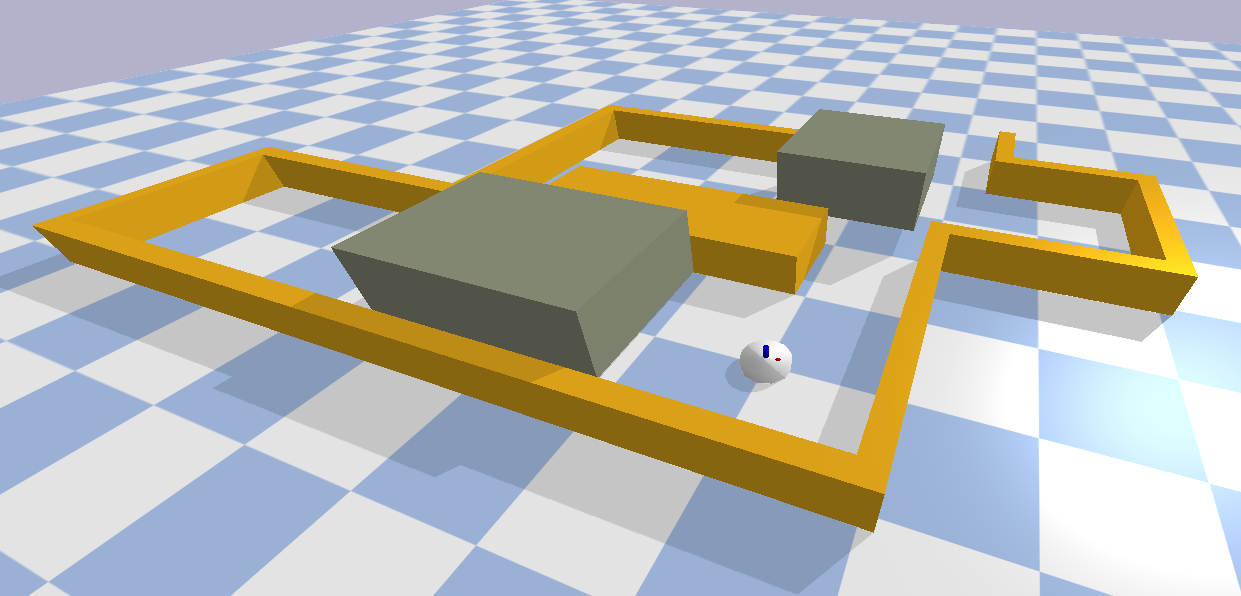
\includegraphics[width=0.8\textwidth]{figures/planning/two_push_to_freedom_env}
    \caption{Environment with the pointrobot, unmovable yellow walls and movable brown boxes.}%
    \label{fig:two_pushes_to_freedom_env}
\end{figure}

The point robot has an cylinderical shape thus a 2 dimensional configuration space is created and can be seen in \cref{fig:two_pushes_to_freedom_conf_space}.

\begin{figure}[H]
  \centering
  \begin{subfigure}{.49\textwidth}
    \centering
    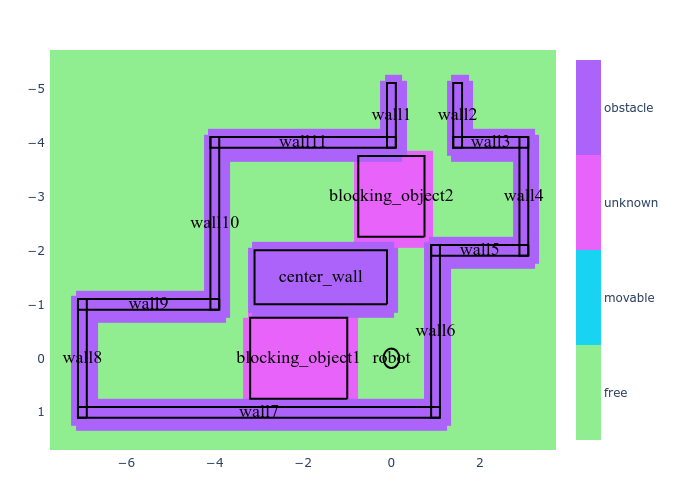
\includegraphics[width=1.05\textwidth]{figures/planning/c_space_point_robot_grid_size_0_1}
    \caption{$\gls{cspace}^{circle}$ with $\gls{cellSize} = 0.1$}%
    \label{fig:c_space_two_pushes_small}
  \end{subfigure}
  \begin{subfigure}{.49\textwidth}
    \centering
    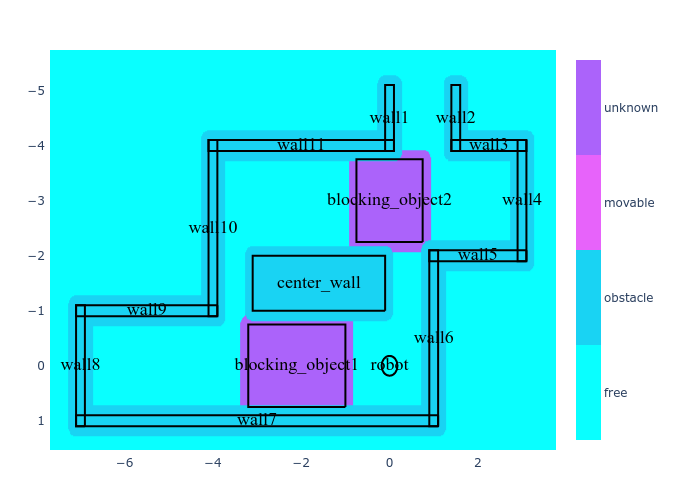
\includegraphics[width=1.05\textwidth]{figures/planning/c_space_point_robot_grid_size_0_01}
    \caption{$\gls{cspace}^{circle}$ with $\gls{cellSize} = 0.01$}%
    \label{fig:c_space_two_pushes_smaller}
  \end{subfigure}
  \caption{The configuration space for the point robot with different cell sizes. The robot\\environment corresponds to the environment presented in \cref{fig:two_pushes_to_freedom_env}.}
  \label{fig:two_pushes_to_freedom_conf_space}
\end{figure}

The resolution of the configuration space at \cref{fig:c_space_two_pushes_smaller} is higher compared to \cref{fig:c_space_two_pushes_small} because of the smaller grid size. The difference in resolution is especially visable at the corners of the walls. A high resolution is better at detecting paths through small quoridors and tight corners, but it comes at the cost of a longer creation and search time.

\paragraph{Path Existence Algorithm}
In context of this thesis we can describe path existence as: \textit{For an object's configuration space there exist an list of neighboring cells from starting to target configuration that do not lie in obstacle space.\bs}

A path in configuration space is detected using the implemented $f_\mathit{shortest\_path}(\gls{c}_\mathit{start}, \gls{c}_\mathit{target}, detect\_blocking\_objects)$ function. This function returns a shortest path from the $\gls{c}_\mathit{start}$ to the $\gls{c}_\mathit{target}$. \textit{detect\_blocking\_objects} is a boolean flag that if \textit{True} returns a list blocking objects that are classified as movable or unknown. If no path can be found, the $f_\textit{shortest\_path}$ function raises an error.\bs

The \textit{shortest\_path} function uses the Dijkstra algorithm 
\cite{dijkstra_note_1959} on the configuration space to find a shortest path. This path can be converted to provide a initial number of samples for motion or manipluation planners, also referreed to as a \quotes{warm start}.

\paragraph{Unfeasible solutions and an undecidable problem}
The path estimation algorithms does not take system constraints into account. It is thus possible that the path estimation algorithm finds a list of neighboring cells from the start to the target configuration and concludes that there exist a path. In reality, this path is unfeasible. An example is driving the boxer robot displayed in \cref{subfig:example_boxer_robot} through a narrow, sharp corner. Whilst geometrically the robot would fit through the corner, the nonholonomic constraints of the robot prevent it from steering through such a thight corner. It is for the motion or manipulation planner to detect that the path is unfeasible.\\

The path estimator suffers from another drawback, finding proof that there exists a path that is undecidable~\cite{zhang_simple_2008}. This is due to the chosen cell size during discretising the configuration space. An example is a quoridor that has exactly the width of the robot, the robot does fit exactly through this quoridor. Detecting such a path requires a number of neighboring cells that lie exactly in the centre line of the quoridor. Only with a cell size going to zero, and the number of cells going to infinity such a path is guaranteed to be detected. Path non-existence on the other hand is more easily to proof, since the path estimation algorithm provides a upper bound on existing paths and a lower bound on non-existing paths~\cite{zhang_simple_2008}.\bs

The path existence algorithm can detect non-existence paths. Thus checking path existence before motion or manipulation planning filters out a number of non-existent paths that would otherwise waste time and resources. Even if in exceptional cases the path estimation algorithm can yield unfeasible paths and can fail to detect existing paths. Checking path existence before motion or manipulation planning filters a number of non-exist paths and is additionally motivated by two reasons. First, because \cref{fig:speed_comparison_planning} shows that an path estimation is orders of magnitudes faster compared to motion or manipulation planning. Secondly, because the path estimation algorithm can provide a number of initial samples to the motion or manipulation planner that can act as a \quotes{warm start}.

\subsection{Motion Planning}%
\label{subsec:motion_planning}
Controllers discussed in \cref{sec:control_methods} can track a path from start to target. Providing a path is the motion planners' responsibility, motion planners seek inside the configuration space for a path from the start to the target configuration. A practical example of such a path is a list of successive robot poses, from starting pose (coinciding with the starting configuration) toward the target pose, where the successive poses lie close together 
\todo[inline]{smsmmsmssm 20 timesamplesThe }
(reachable for the robot in $\sim20$ time samples). Seeking a path from start to target inside a configuration space whilst avoiding obstacles for the robot to track is referred to as \textit{motion planning}. Finding a path between the start and target configuration for pushing applications whilst avoiding collisions is referred to as \textit{manipulation planning}. First, this subsection presents motion planning, and the next subsection \cref{subsec:manipulation_planning} dedicates itself to manipulation planning. For both motion and manipulation planning and sampling-based methods are used, which can be described as.\bs

\textit{\quotes{The main idea is to avoid the explicit construction of the object space, and instead conduct a search that probes the configuration space with a sampling scheme. This probing is enabled by a collision detection module, which the motion planning algorithm considers as a “black box.”~\cite{lavalle_planning_2006}}}\bs

Generally, the configuration space motion planners plan consists of 2 subspaces, free and obstacle space. The configuration space in this thesis consists of 4 subspaces, namely free, obstacle, unknown and movable space. To solve motion planning problems for such a configuration space a dedicated motion planning algorithm has been developed that extends the existing algorithm extends the existing double tree \ac{RRT*} algorithm~\cite{chen_fast_2018}. The motion planner consists of.
\begin{center}
\begin{tabular}[t]{l p{10cm}}
$V$:& A set of nodes\\
$E$:& A set of edges\\
$P$:& A set of paths\\
\end{tabular}
\end{center}

The start connectivity tree consists of the nodes connected by edges containing the starting node, and vice versa for the target connectivity tree containing the target node. The algorithm grows the two \textit{connectivity trees} by randomly sampling configurations and adding them to the start or target connectivity tree. The algorithm explores configuration space by growing these connectivity trees. When the start connectivity tree meets the target connectivity tree a path from start to target is found.\bs

Newly sampled configurations are added in a structural manner that guarantees an optimal path is found with infinite sampling. Where optimality is defined as the path with the lowest cost.

\todo[inline]{Corrado: This is also your idea right? If you put it like this it sounds like it’s common practice from the literature }

The cost is defined as a sum of a distance metric and a fixed penalty for paths that cross unknown or movable subspaces. Incentivising the algorithm to find a path around unknown or movable obstacles over a path crossing through unknown or movable obstacles.\bs

The algorithm takes in 2 arguments, first the \textit{step size}, the maximal normalised distance between connected samples in the connectivity trees. Second, the \textit{search size} is a subspace around newly sampled samples, inside this subspace a parent node is saught that results in the lowest cost, rewiring of closeby nodes happens and the other connectivity tree is searched to detect a full path from start to target.\bs

Now pseudocode of the proposed algorithm is provided in \cref{pseudocode:proposed_rrt_star}, and functions used are elaborated on in \cref{table:functions_for_proposed_rrt_star}. The coloured sections inside \cref{pseudocode:proposed_rrt_star} correspond to the surrounding coloured box around subfigures in \cref{fig:motion_planner_adding_one_sample}. The following definitions are used by the proposed algorithm.\bs

\todo[inline]{It is a suprise to suddenly read that there apparently is a "proposed algorithm". The chapter/section intro doesn't mention that something will be proposed, and neither does all of the text leading up to this sentence.}


\begin{table}[H]
\centering
\begin{tabular}[t]{l p{10cm}}
$x$:& A node containing a point in configuration space\\
$x_{init}$:& Creates a start and target node\\ 
$NotReachStop$:& True if the stopping criteria is not reached\\ 
$Sample_{random}$:& Creates a random sample in free-, movable- or unknown space\\
$Nearest(x, V)$:& Returns the nearest nodes from $x$ in $V$\\
$NearestSet(x, V)$:& Returns set of nearest nodes from $x$ in $V$\\
$Project(x, x')$:& Project $x$ toward $x'$\\
$CollisionCheck(x)$:& Returns true if $x$ is in free-, movable- or unknown space\\
$ObjectCost(x', x)$:& Returns a fixed additional cost if $x$ enters movable- or unknown space from $x'$, otherwise returns 0\\
$Distance(x, x')$:& Returns the distance between sample $x$ and $x'$\\
$CostToInit(x)$:& Find the total cost from $x$ to the initial node\\
$LocalPlannerCheck(x, x')$:& Return true if a local planner is able to connect $x$ and $x'$, otherwise return false. A system model (see \cref{sec:sys_iden}) acts a local planner\\
$InSameTree(x, x')$:& Returns true if both $x$ and $x'$ are in the same tree, otherwise return false\\
\end{tabular}
\caption{Functions used by the \cref{pseudocode:proposed_rrt_star}}
\label{table:functions_for_proposed_rrt_star}
\end{table}

\todo[inline]{you did not yet say anithing about modified RRT, stop that}
\newpage
\begin{algorithm}[H]
\caption{Pseudocode for modified $\text{RRT}^*$ algorithm taking movable objects and constraints into account}
\label{pseudocode:proposed_rrt_star}
\begin{algorithmic}[1]

\hspace{-0.9cm}\colorbox{my_grey}{\parbox{\linewidth}{%
\State $V \leftarrow x_{init}$
\While{$NotReachStop$} 

\hspace{-0.1cm}\colorbox{my_light_blue}{\parbox{\linewidth}{%
    \State $Cost_{min} \leftarrow +\infty$ \algorithmiccomment{Create, check and project a new random sample}
    \State $x_{rand} \leftarrow Sample_{random}$
    \State $x_{nearest} \leftarrow Nearest(x_{rand}, V)$
    \State $x_{temp} \leftarrow Project(x_{rand}, x_{nearest})$

    \If{$CollisionCheck(x_{temp})$}
        \State $x_{new} = x_{temp}$
        \Else
        \State $Continue$
    \EndIf
}}

\hspace{-0.1cm}\colorbox{my_yellow}{\parbox{\linewidth}{%
    \State $X_{near} \leftarrow NearestSet(x_{new}, V)$ \algorithmiccomment{Find and connect new node to parent node}
    \For{$x_{near} \in X_{near}$}
    \State $Cost_{temp} \leftarrow CostFromInit(x_{near}) + Distance(x_{near}, x_{new}) + ObjectCost(x_{near}, x_{new})$
    \If{$Cost_{temp}  < Cost_{min}$}
            \If{$LocalPlannerCheck(x_{new}, x_{near})$}
            \State $Cost_{min} \leftarrow x_{temp}$
            \State $x_{minCost} \leftarrow x_{near}$
            \EndIf
        \EndIf
    \EndFor
    \If{$Cost_{min} == \infty$}
        \State $Continue$
    \Else
        \State $V.add(x_{new})$
        \State $E.add(x_{minCost}, x_{new})$
    \EndIf
}}

\hspace{-0.1cm}\colorbox{my_green}{\parbox{\linewidth}{%
    \State $Cost_{path} \leftarrow +\infty$ \algorithmiccomment{Check if the newly added node can lower cost for nearby nodes}
    \For{$x_{near} \in X_{near}$} 
      \If{$InSameTree(x_{near}, x_{new})$} 
        \State $Cost_{temp} \leftarrow CostFromInit(x_{new}) + distance(x_{new}, x_{near}) + ObjectCost(x_{new}, x_{near})$
        \If{$Cost_{temp} < CostFromInit(x_{near})$}
           \If{$LocalPlannerCheck(x_{new}, x_{near})$}
              \State $E.rewire(x_{near}, x_{new})$
           \EndIf
        \EndIf
      \Else \algorithmiccomment{Add lowest cost path to list of paths}
          \State $Cost_{temp} \leftarrow CostFromInit(x_{new}) + distance(x_{new}, x_{near}) $ \newline\hspace*{10em} $+ CostFromInit(x_{near}) + ObjectCost(x_{new}, x_{near})$
          \If{$Cost_{temp}  < Cost_{path}$}
              \If{$LocalPlannerCheck(x_{new}, x_{near})$}
                  \State $Cost_{pathMin} \leftarrow x_{temp}$
                  \State $x_{pathMin} \leftarrow x_{near}$
              \EndIf
          \EndIf
      \EndIf
      \If{$Cost_{pathMin} == \infty$}
          \State $Continue$
      \Else
          \State $P.addPath(x_{new}, x_{pathMin}, Cost_{pathMin})$
      \EndIf
    \EndFor
}}

\EndWhile
}}
\end{algorithmic}
\end{algorithm}

\newpage
Now an example is provided of the proposed algorithm that creates and adds one sample in \cref{fig:motion_planner_adding_one_sample}. After adding the newly sampled sample is added to the start connectivity tree, a sample is rewired then the target connectivity tree is connected to the start connectivity tree. The resulting path found can be visualised in \cref{fig:motion_planner_comparison}.\bs

\begin{figure}[H]
    \centering
    \begin{subfigure}{.49\textwidth}
    \centering
    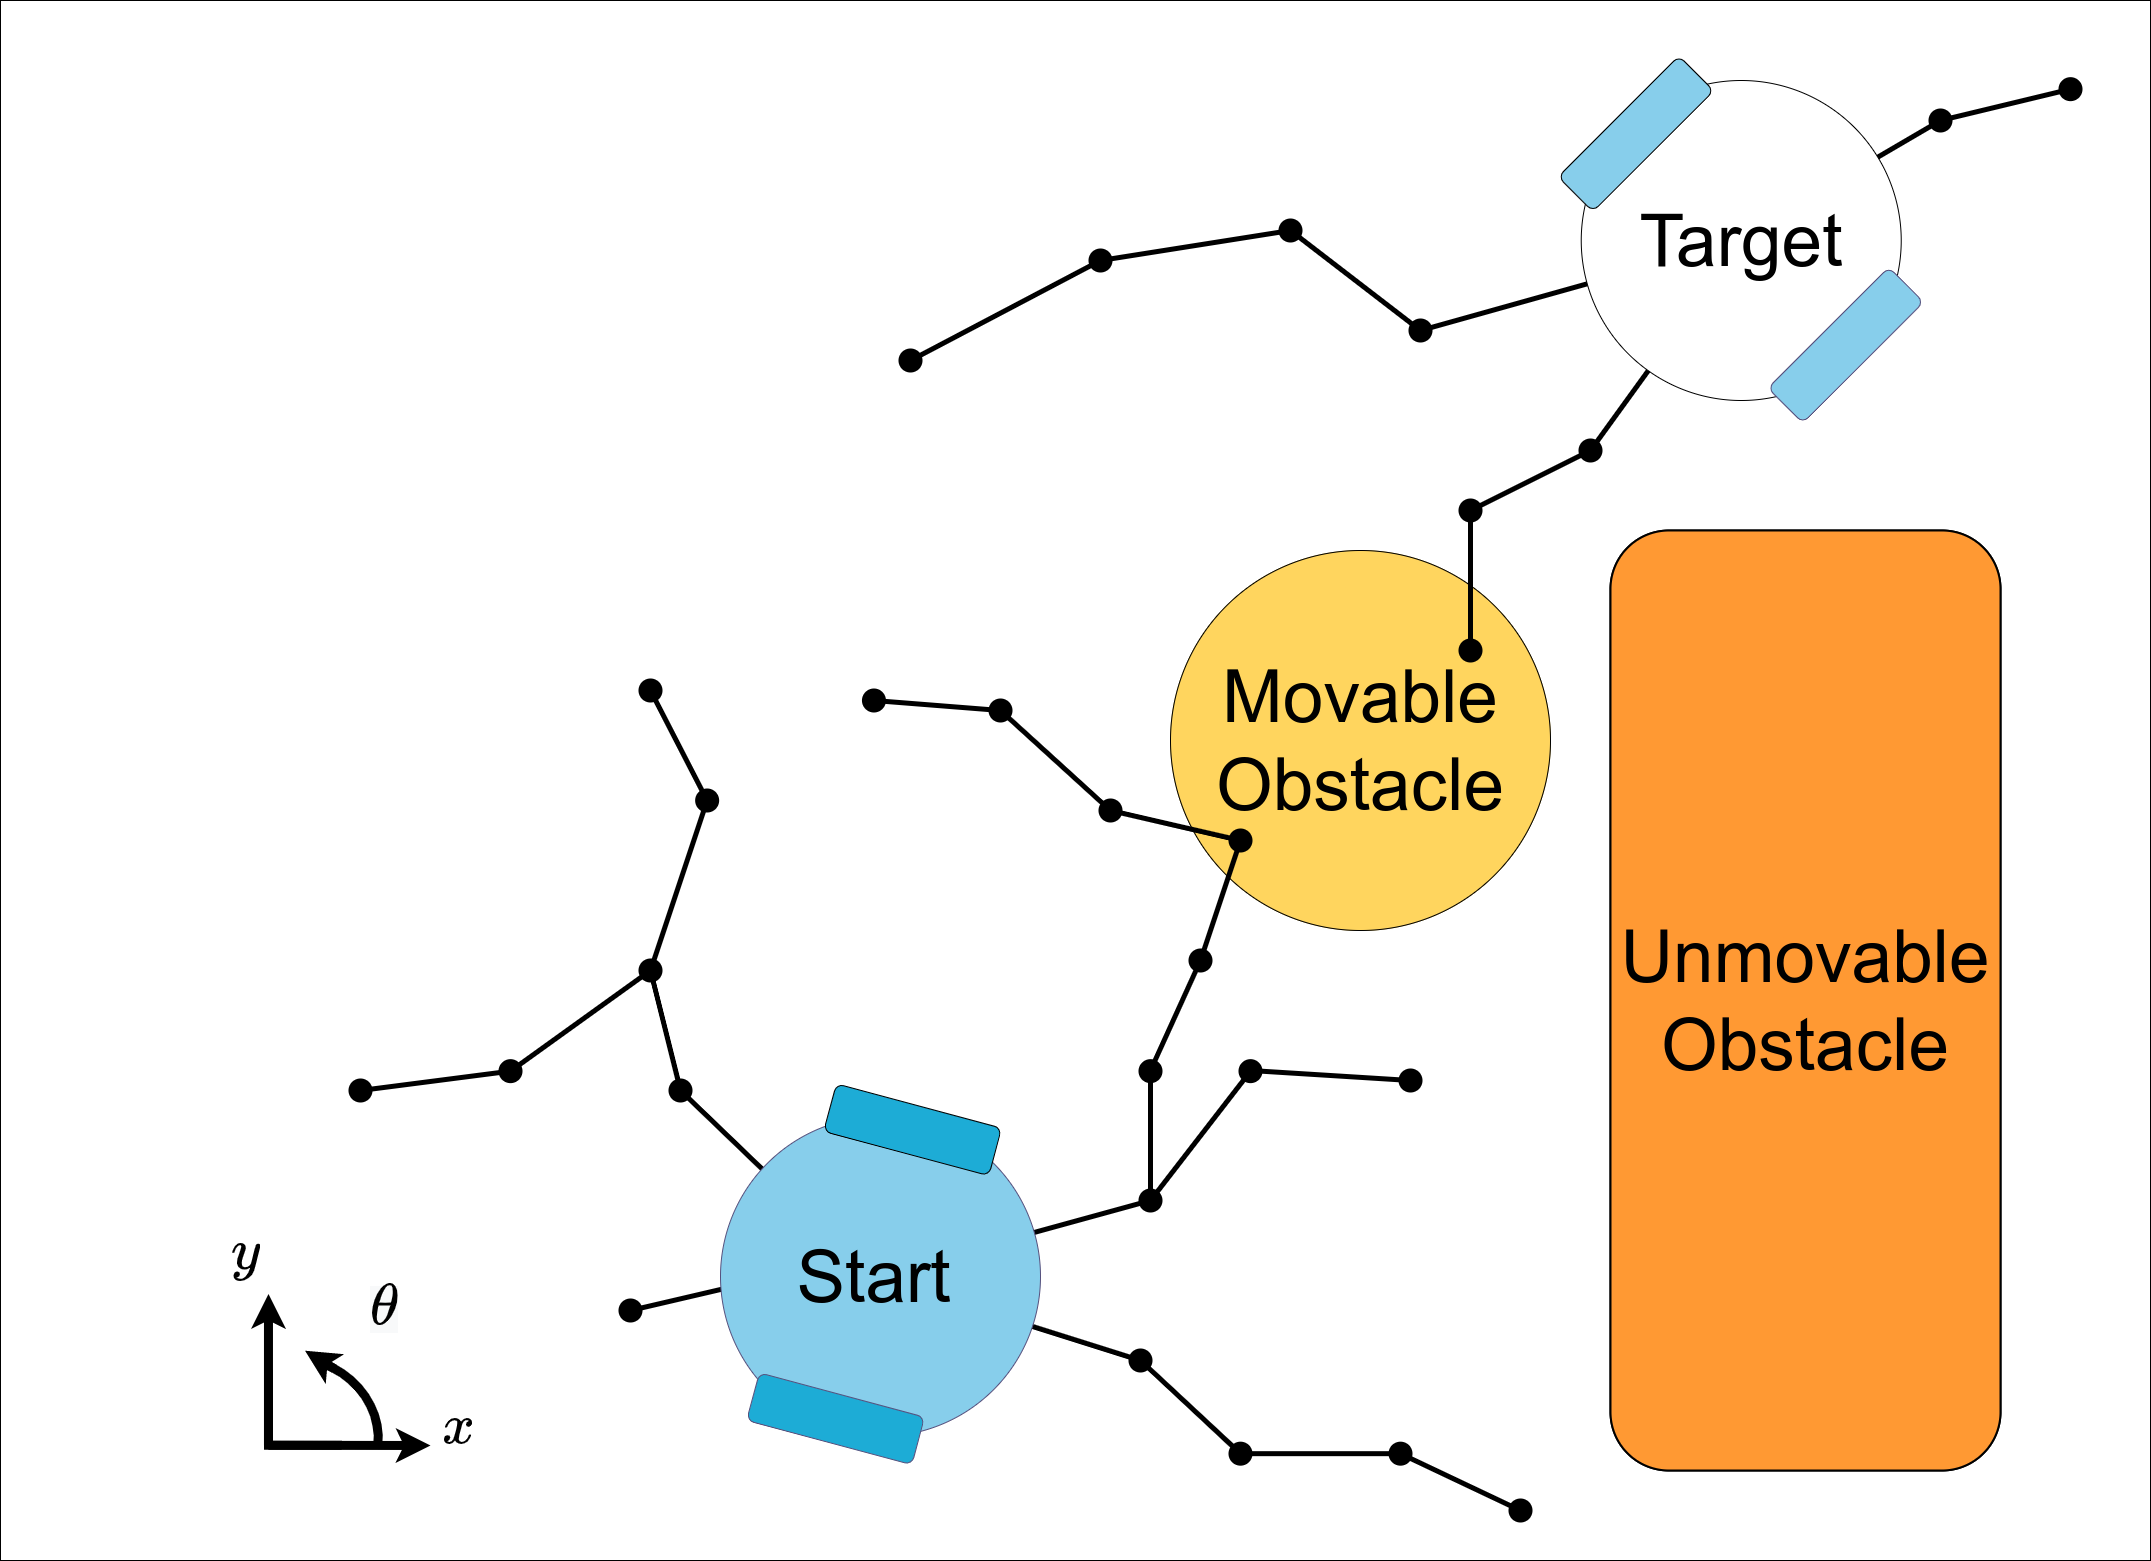
\includegraphics[width=0.93\textwidth, cfbox=my_grey 5pt 0pt]{figures/mp/1mp_init.drawio.png}
    \caption{Snapshot of the configuration space during a search\\from start to the target configuration.}
    \end{subfigure}
    \begin{subfigure}{.49\textwidth}
    \centering
    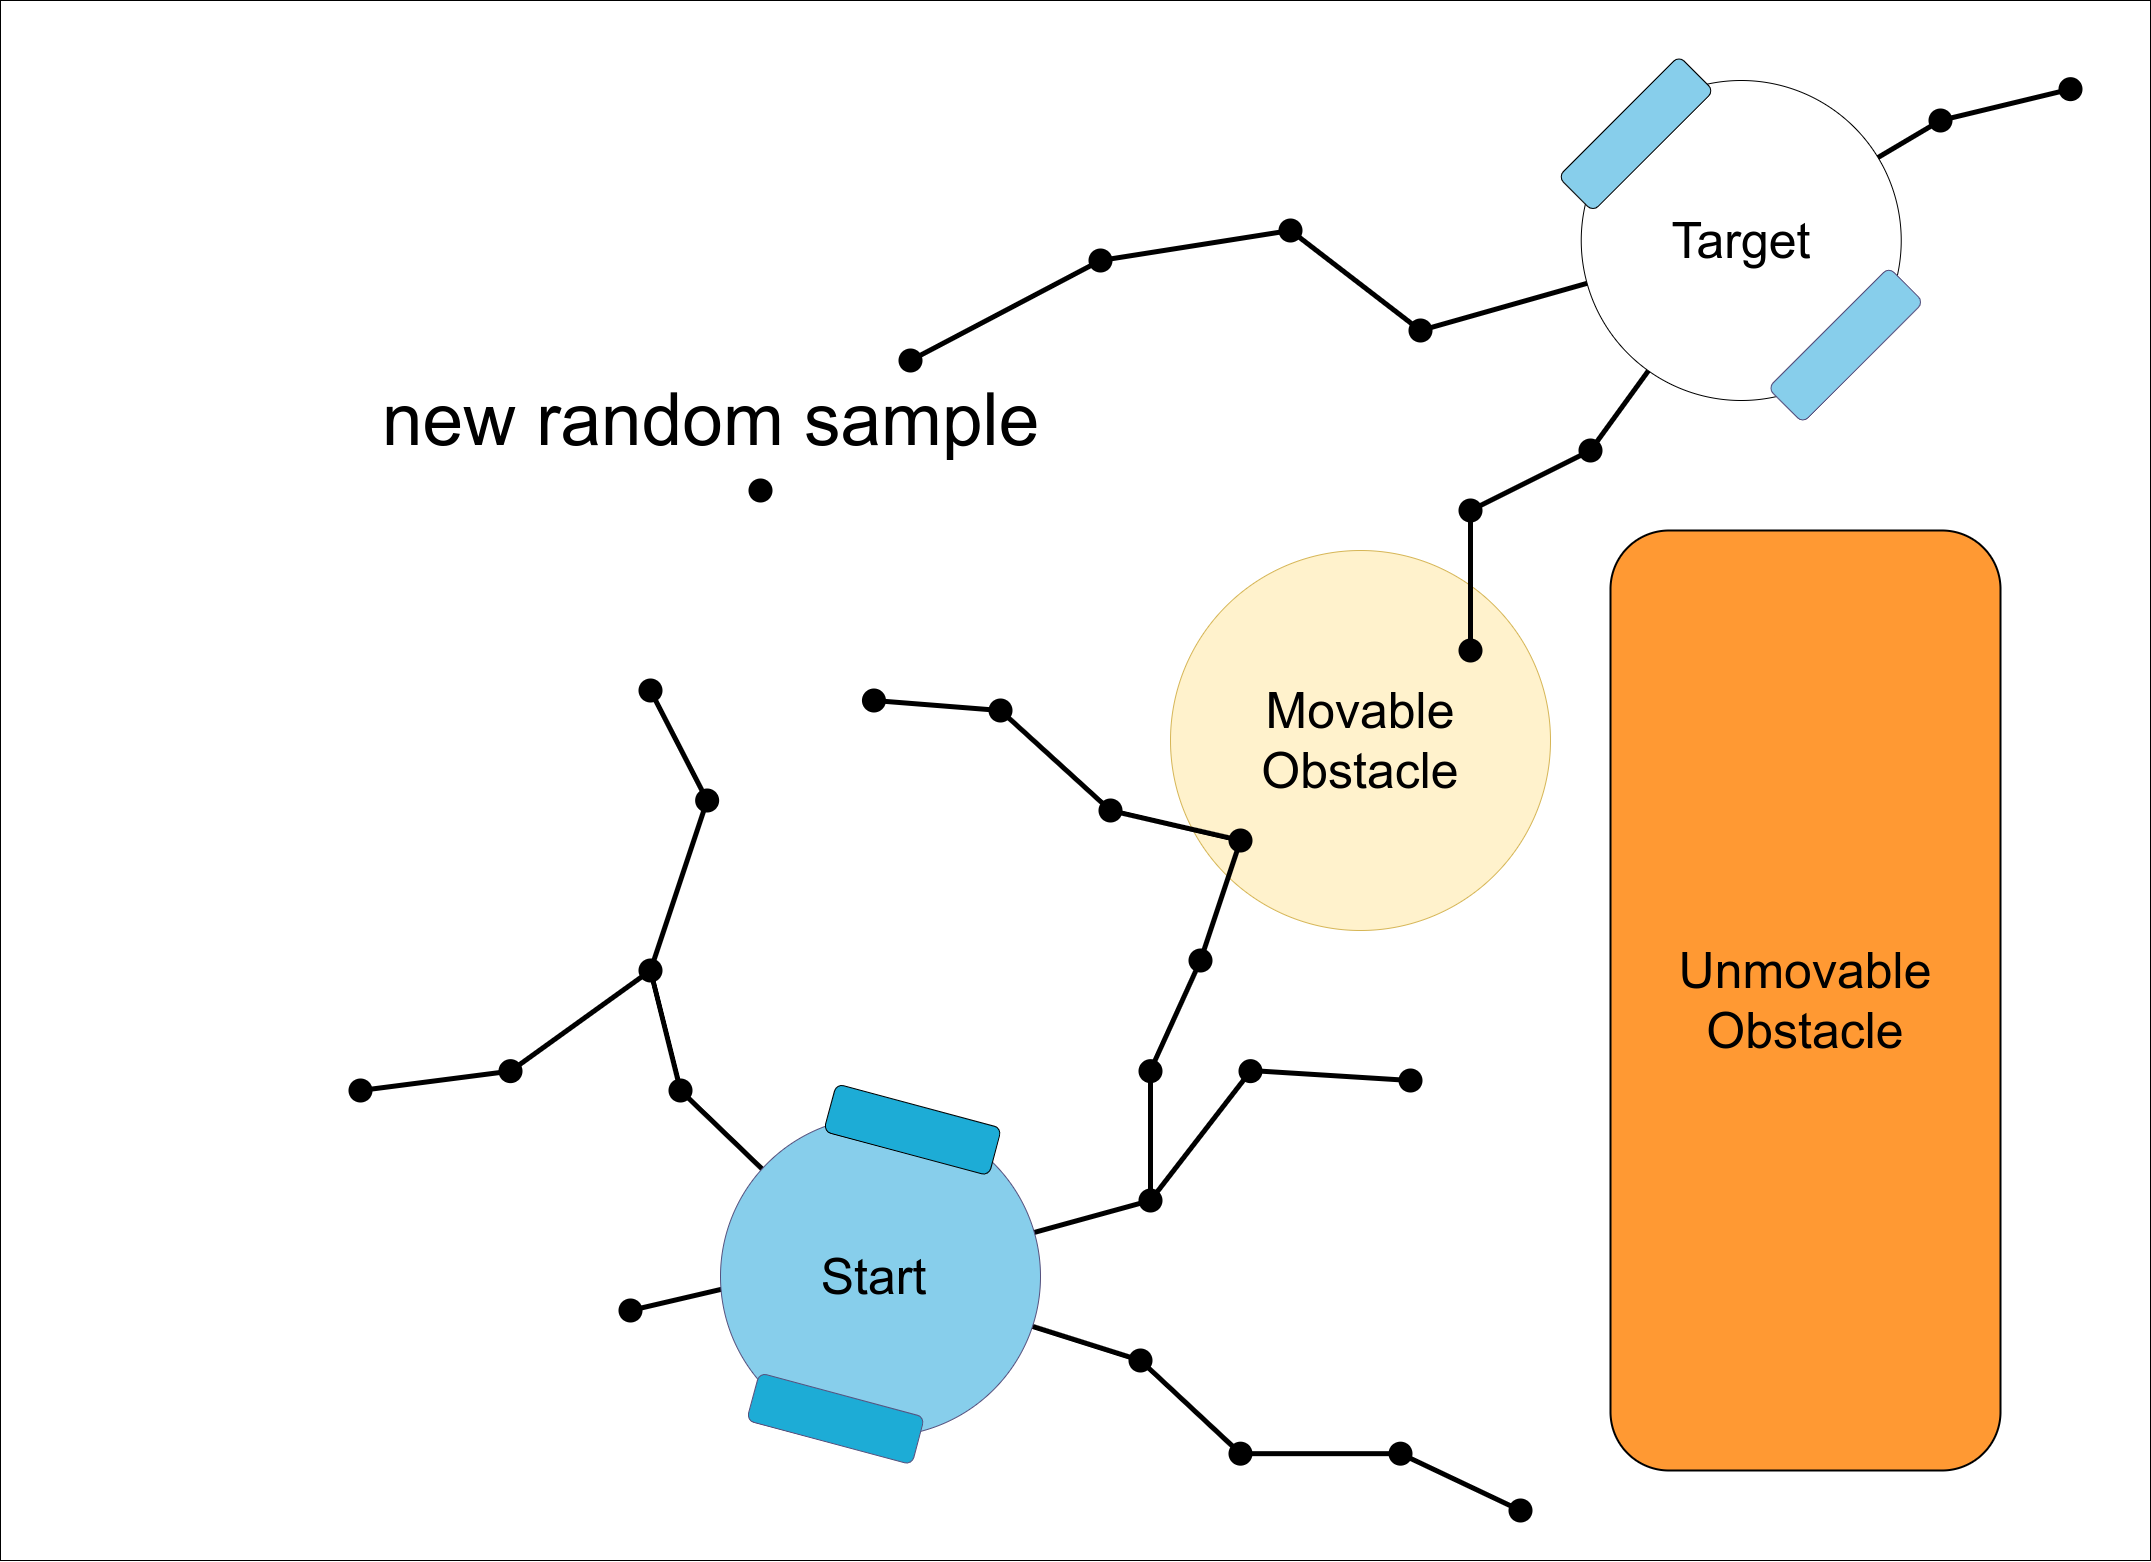
\includegraphics[width=0.93\textwidth, cfbox=my_light_blue 5pt 0pt]{figures/mp/2mp_new_rand_sample.drawio.png}
    \caption{A new random sample is generated.\bs}
    \end{subfigure}

    \begin{subfigure}{.49\textwidth}
    \centering
    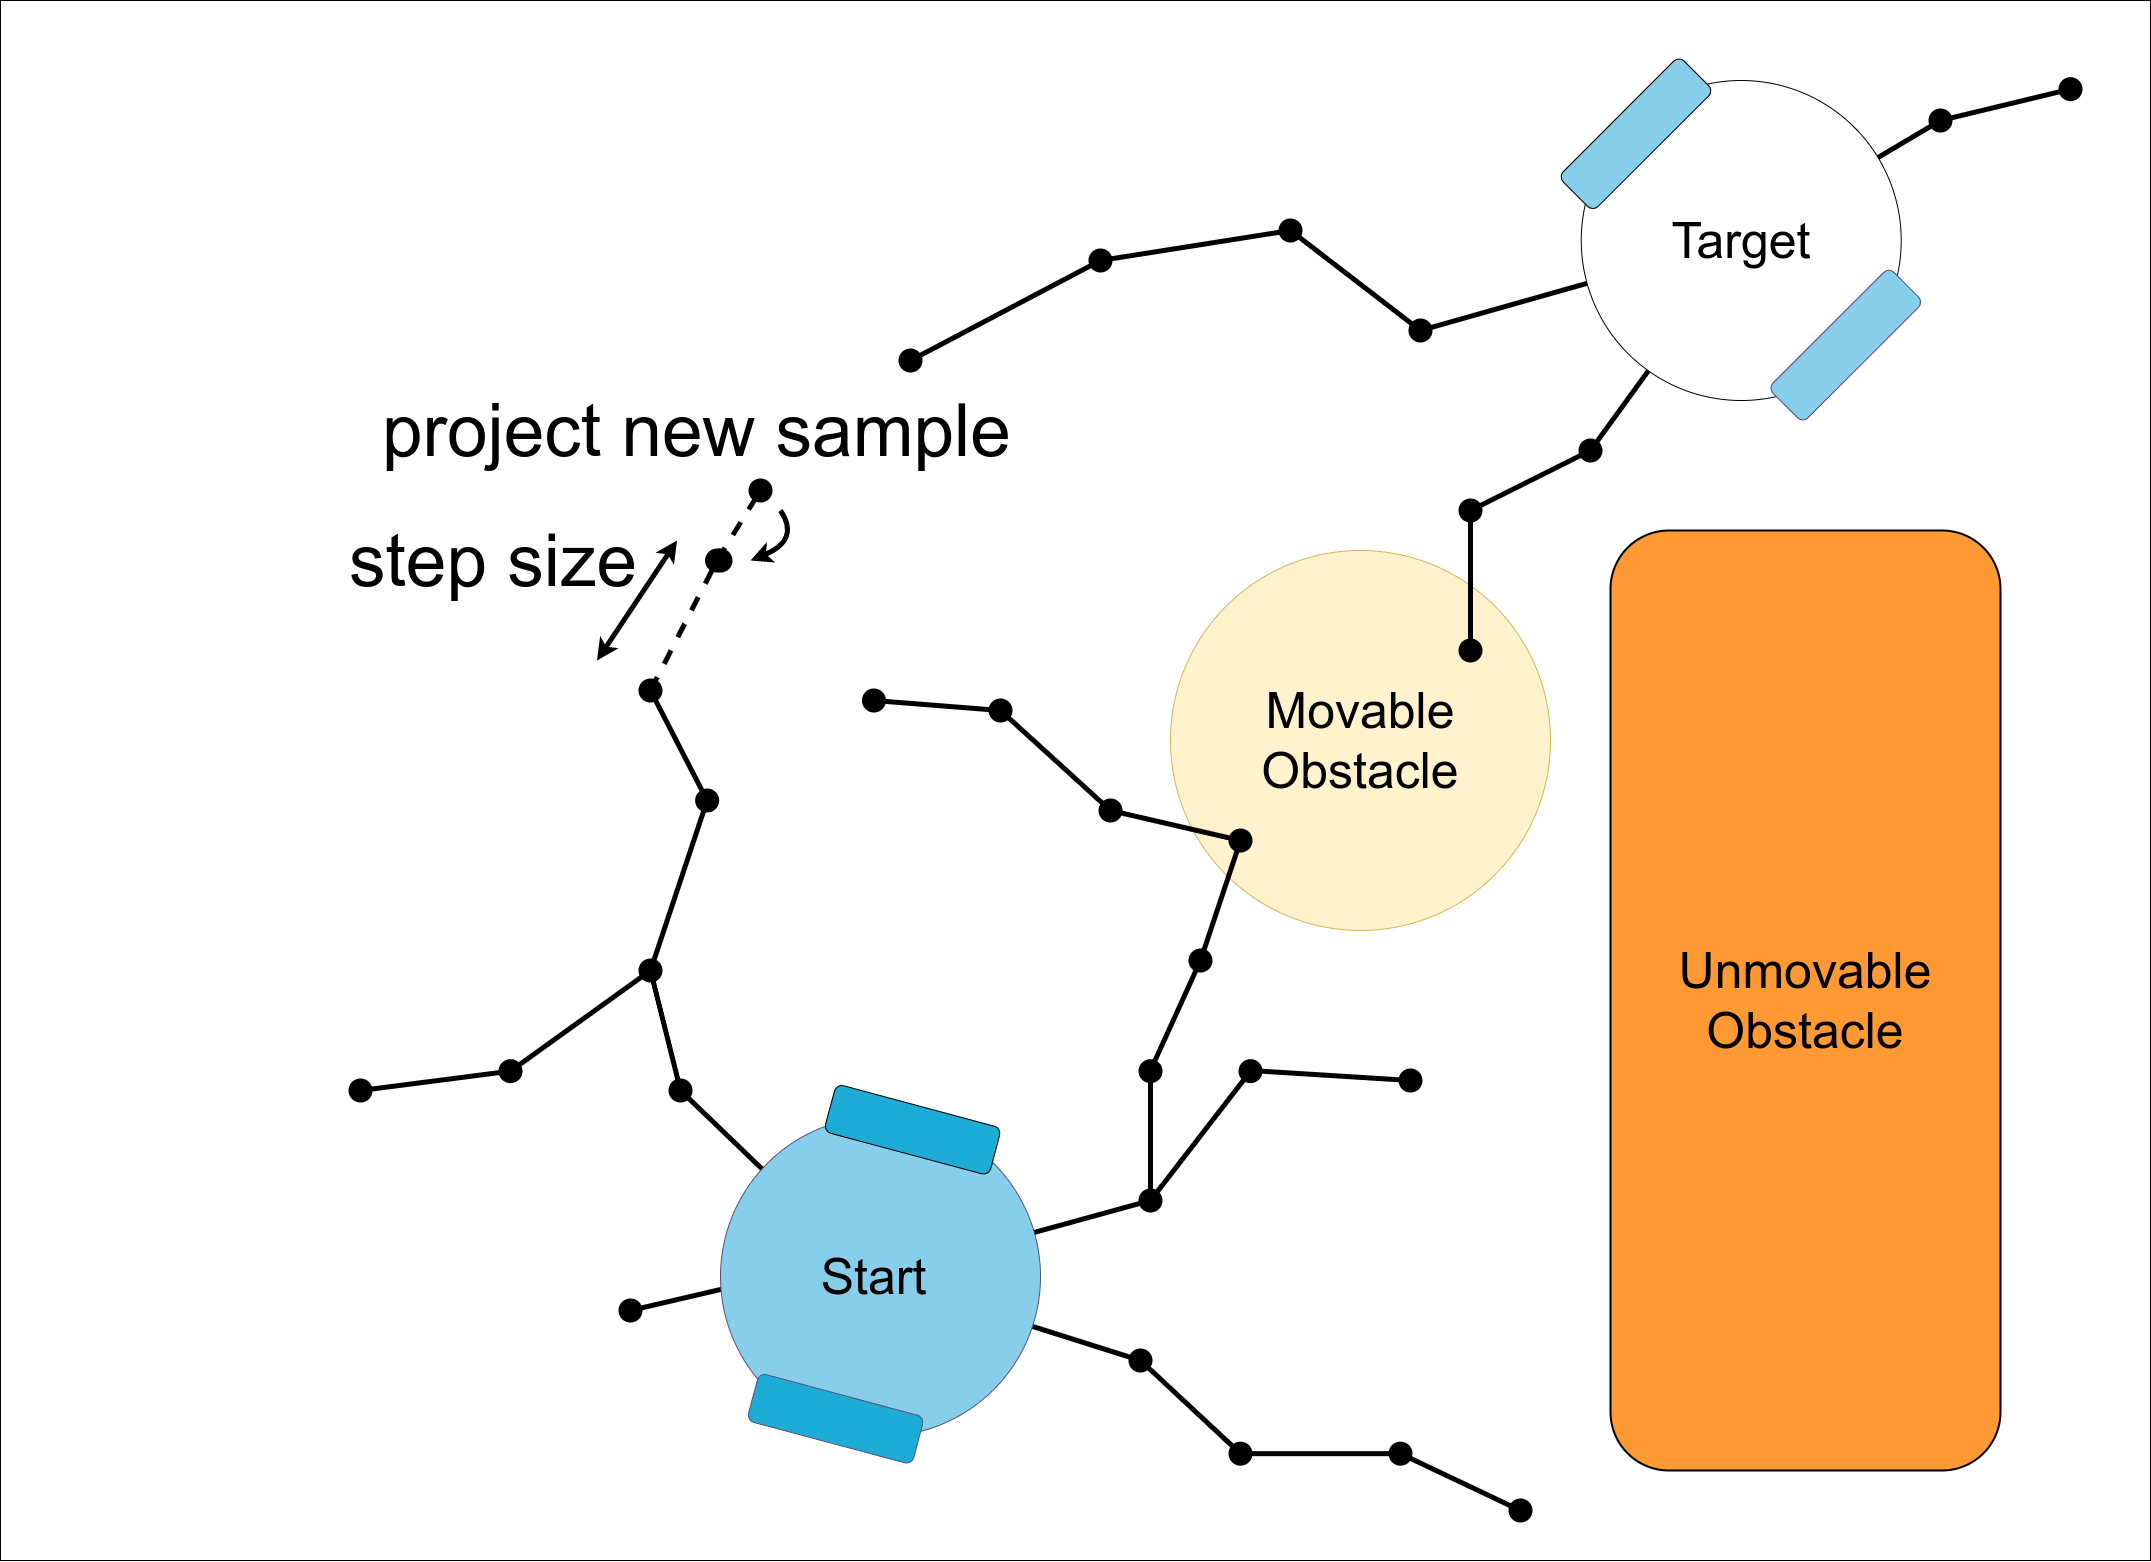
\includegraphics[width=0.93\textwidth, cfbox=my_light_blue 5pt 0pt]{figures/mp/3mp_project_sample.drawio.png}
    \caption{The new sample is projected toward the closest sample.\bs}
    \end{subfigure}
    \begin{subfigure}{.49\textwidth}
    \centering
    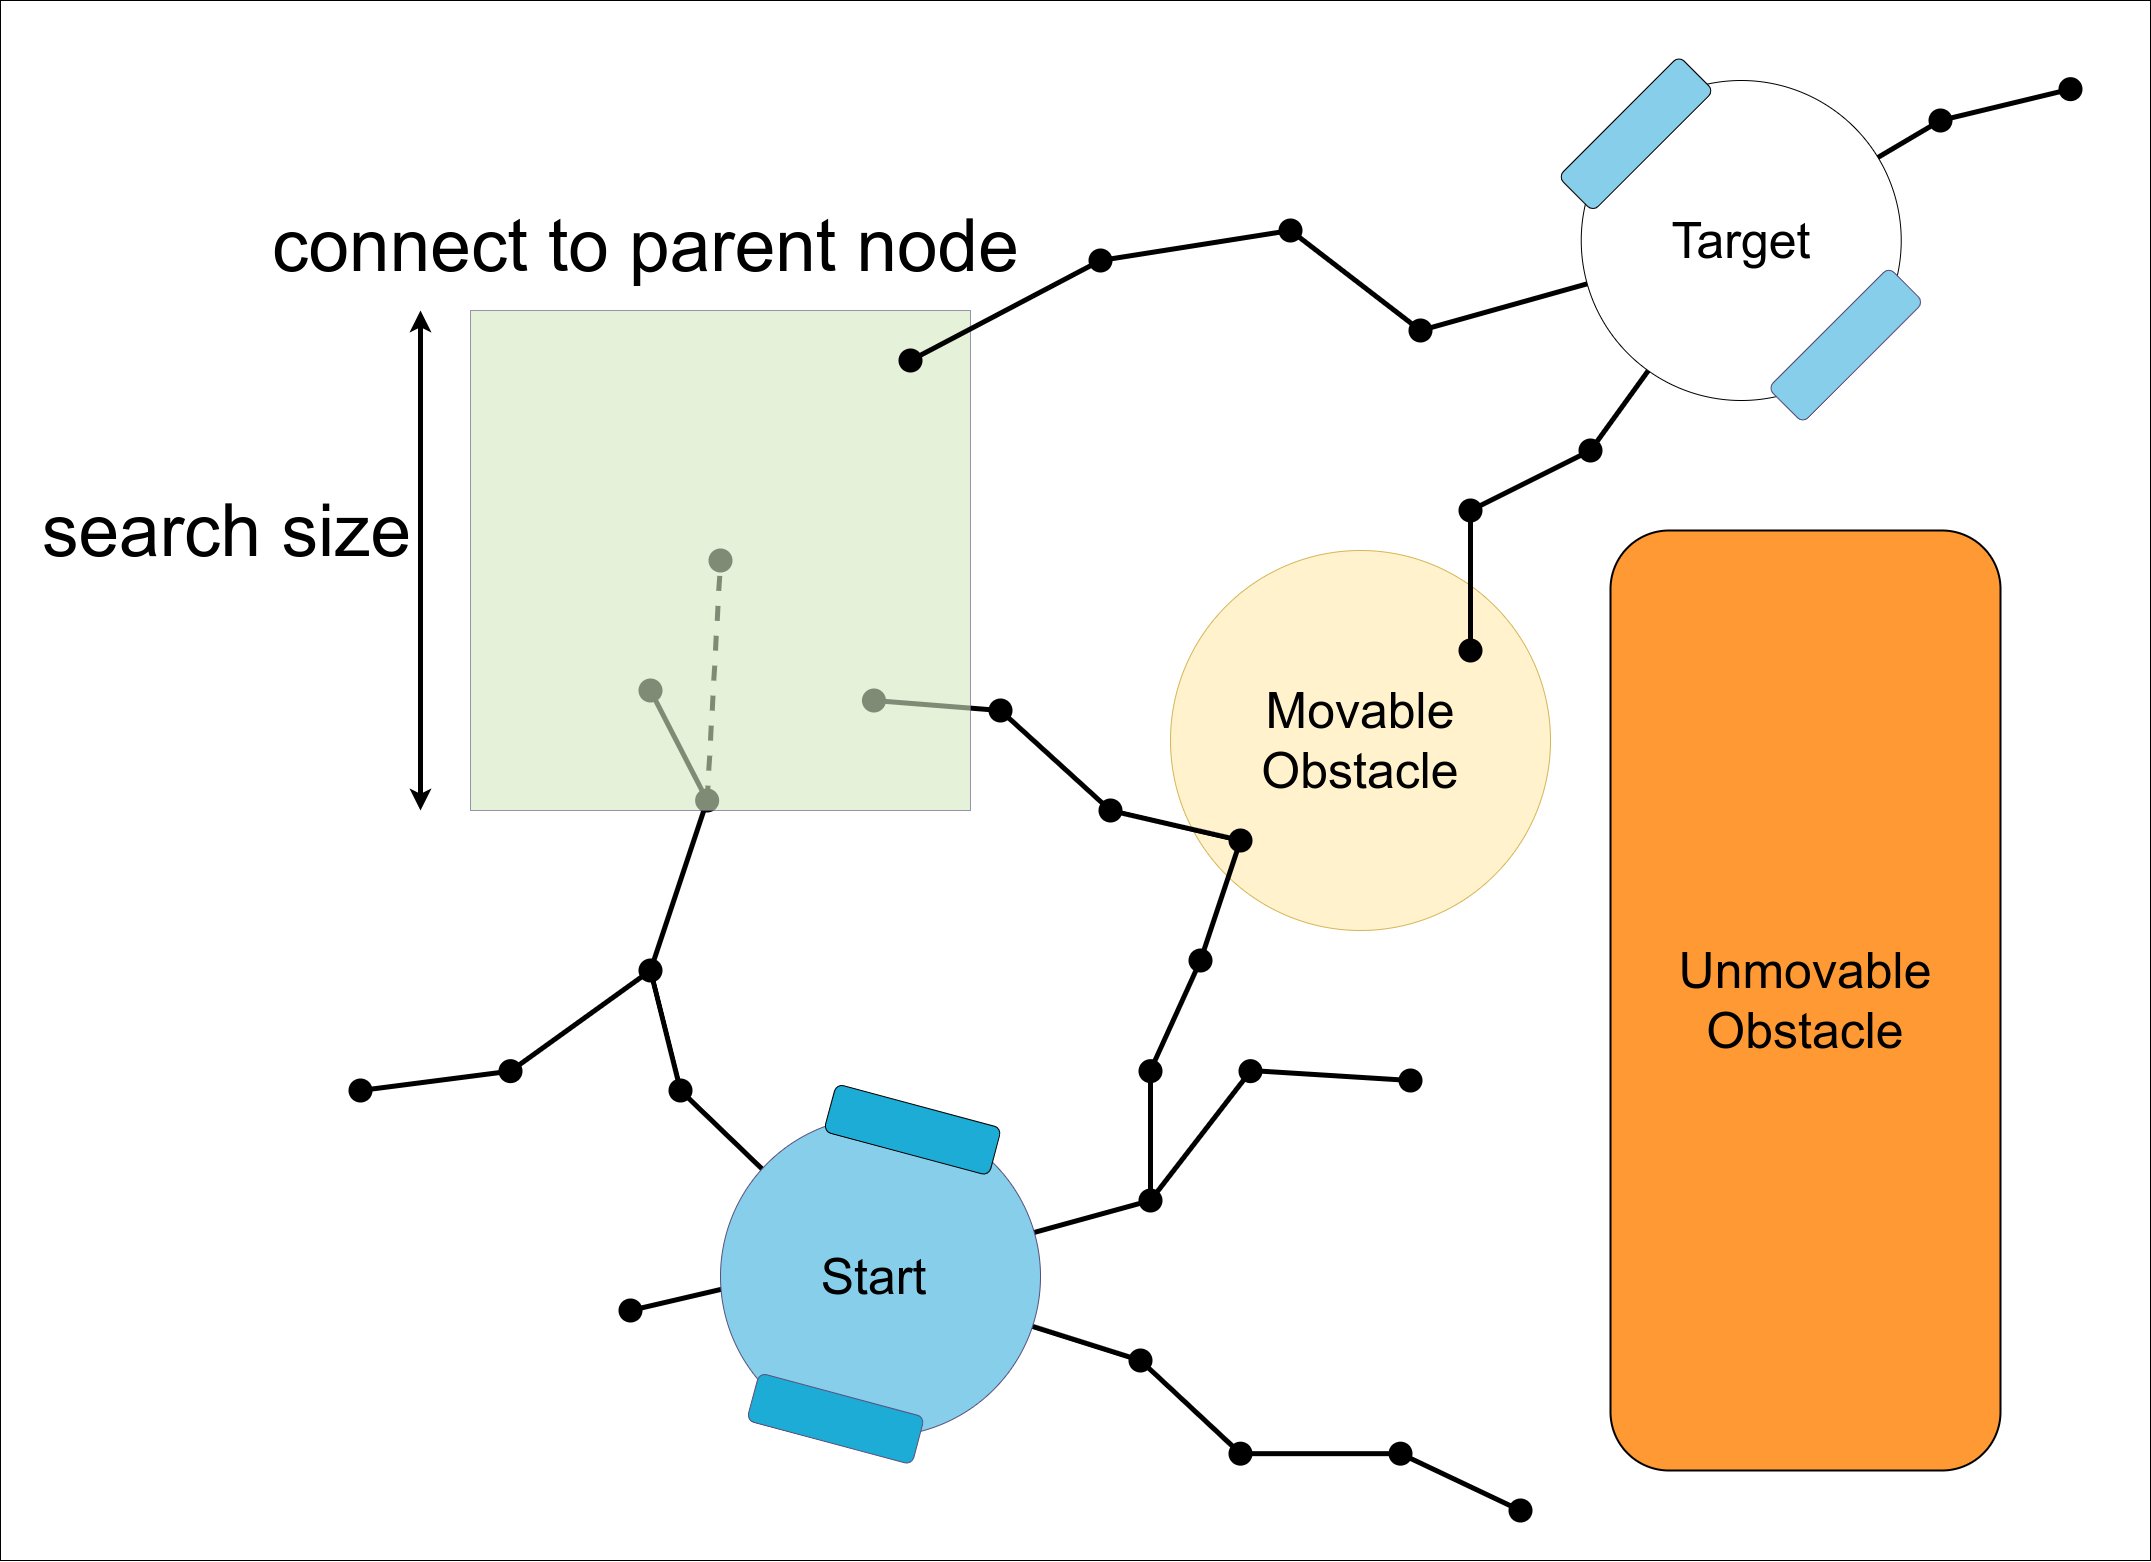
\includegraphics[width=0.93\textwidth, cfbox=my_yellow 5pt 0pt]{figures/mp/4mp_connect_to_tree.drawio.png}
    \caption{The new sample is connected to the node in search space\\that results in the lowest cost.}
    \end{subfigure}

    \begin{subfigure}{.49\textwidth}
    \centering
    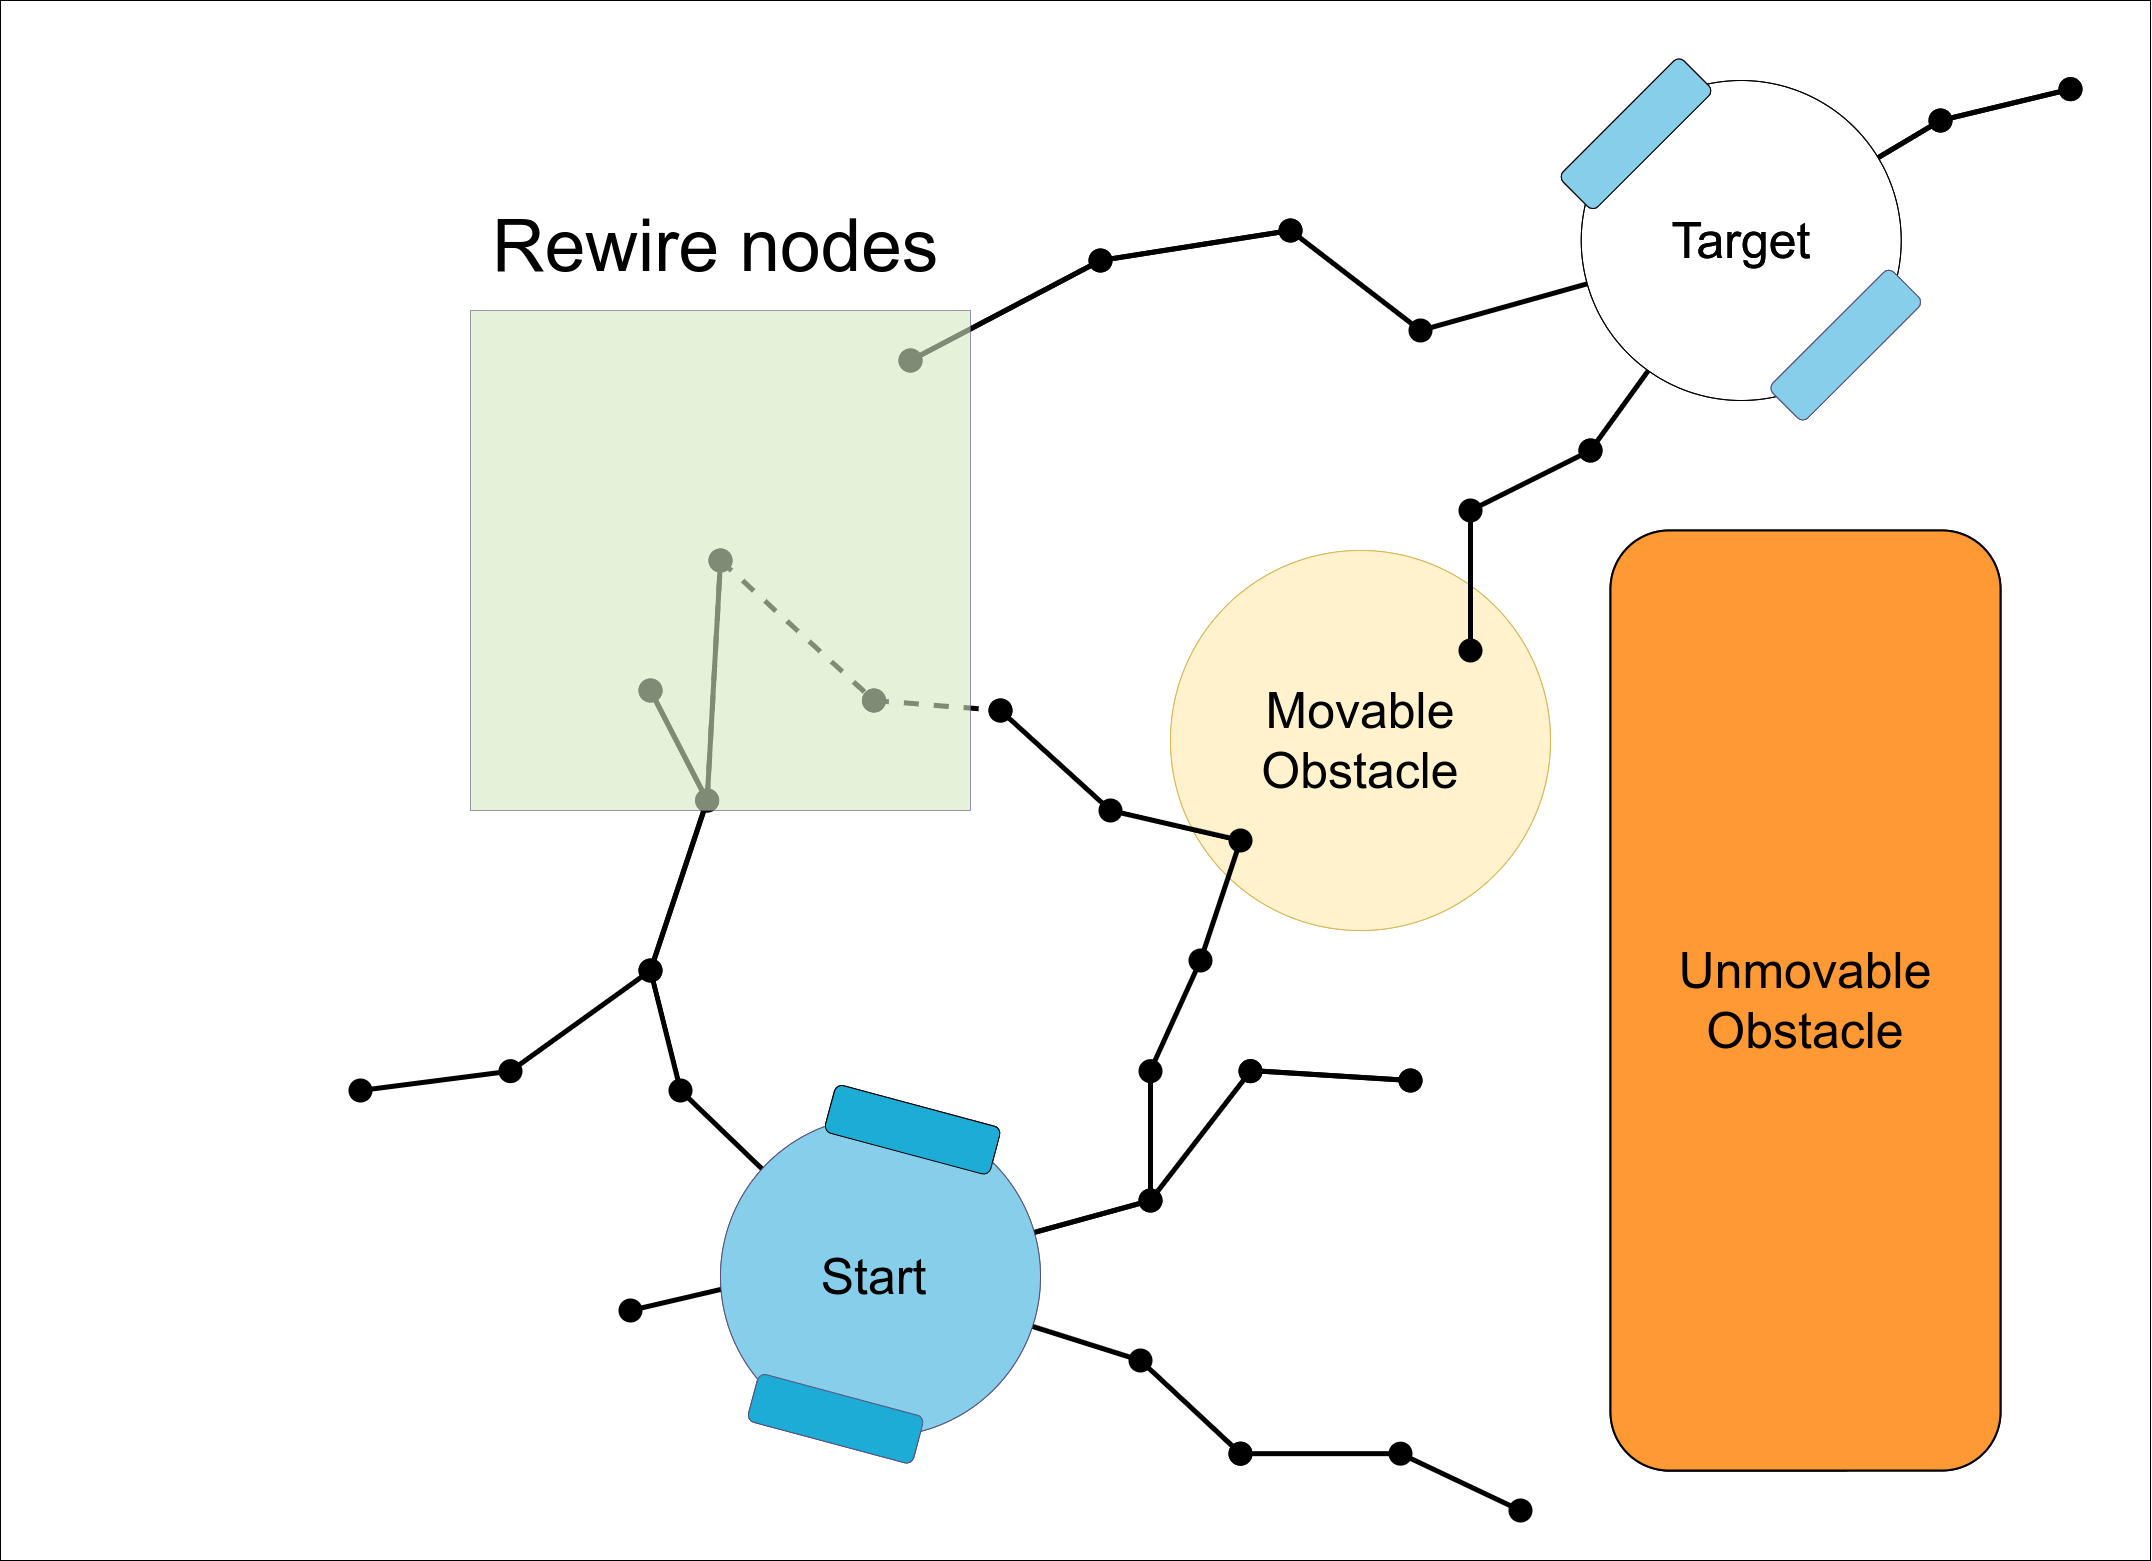
\includegraphics[width=0.93\textwidth, cfbox=my_green 5pt 0pt]{figures/mp/5mp_rewire.drawio.png}
    \caption{Nodes for which the cost can be lowered\\from the new sample are rewired.}
    \end{subfigure}
    \begin{subfigure}{.49\textwidth}
    \centering
    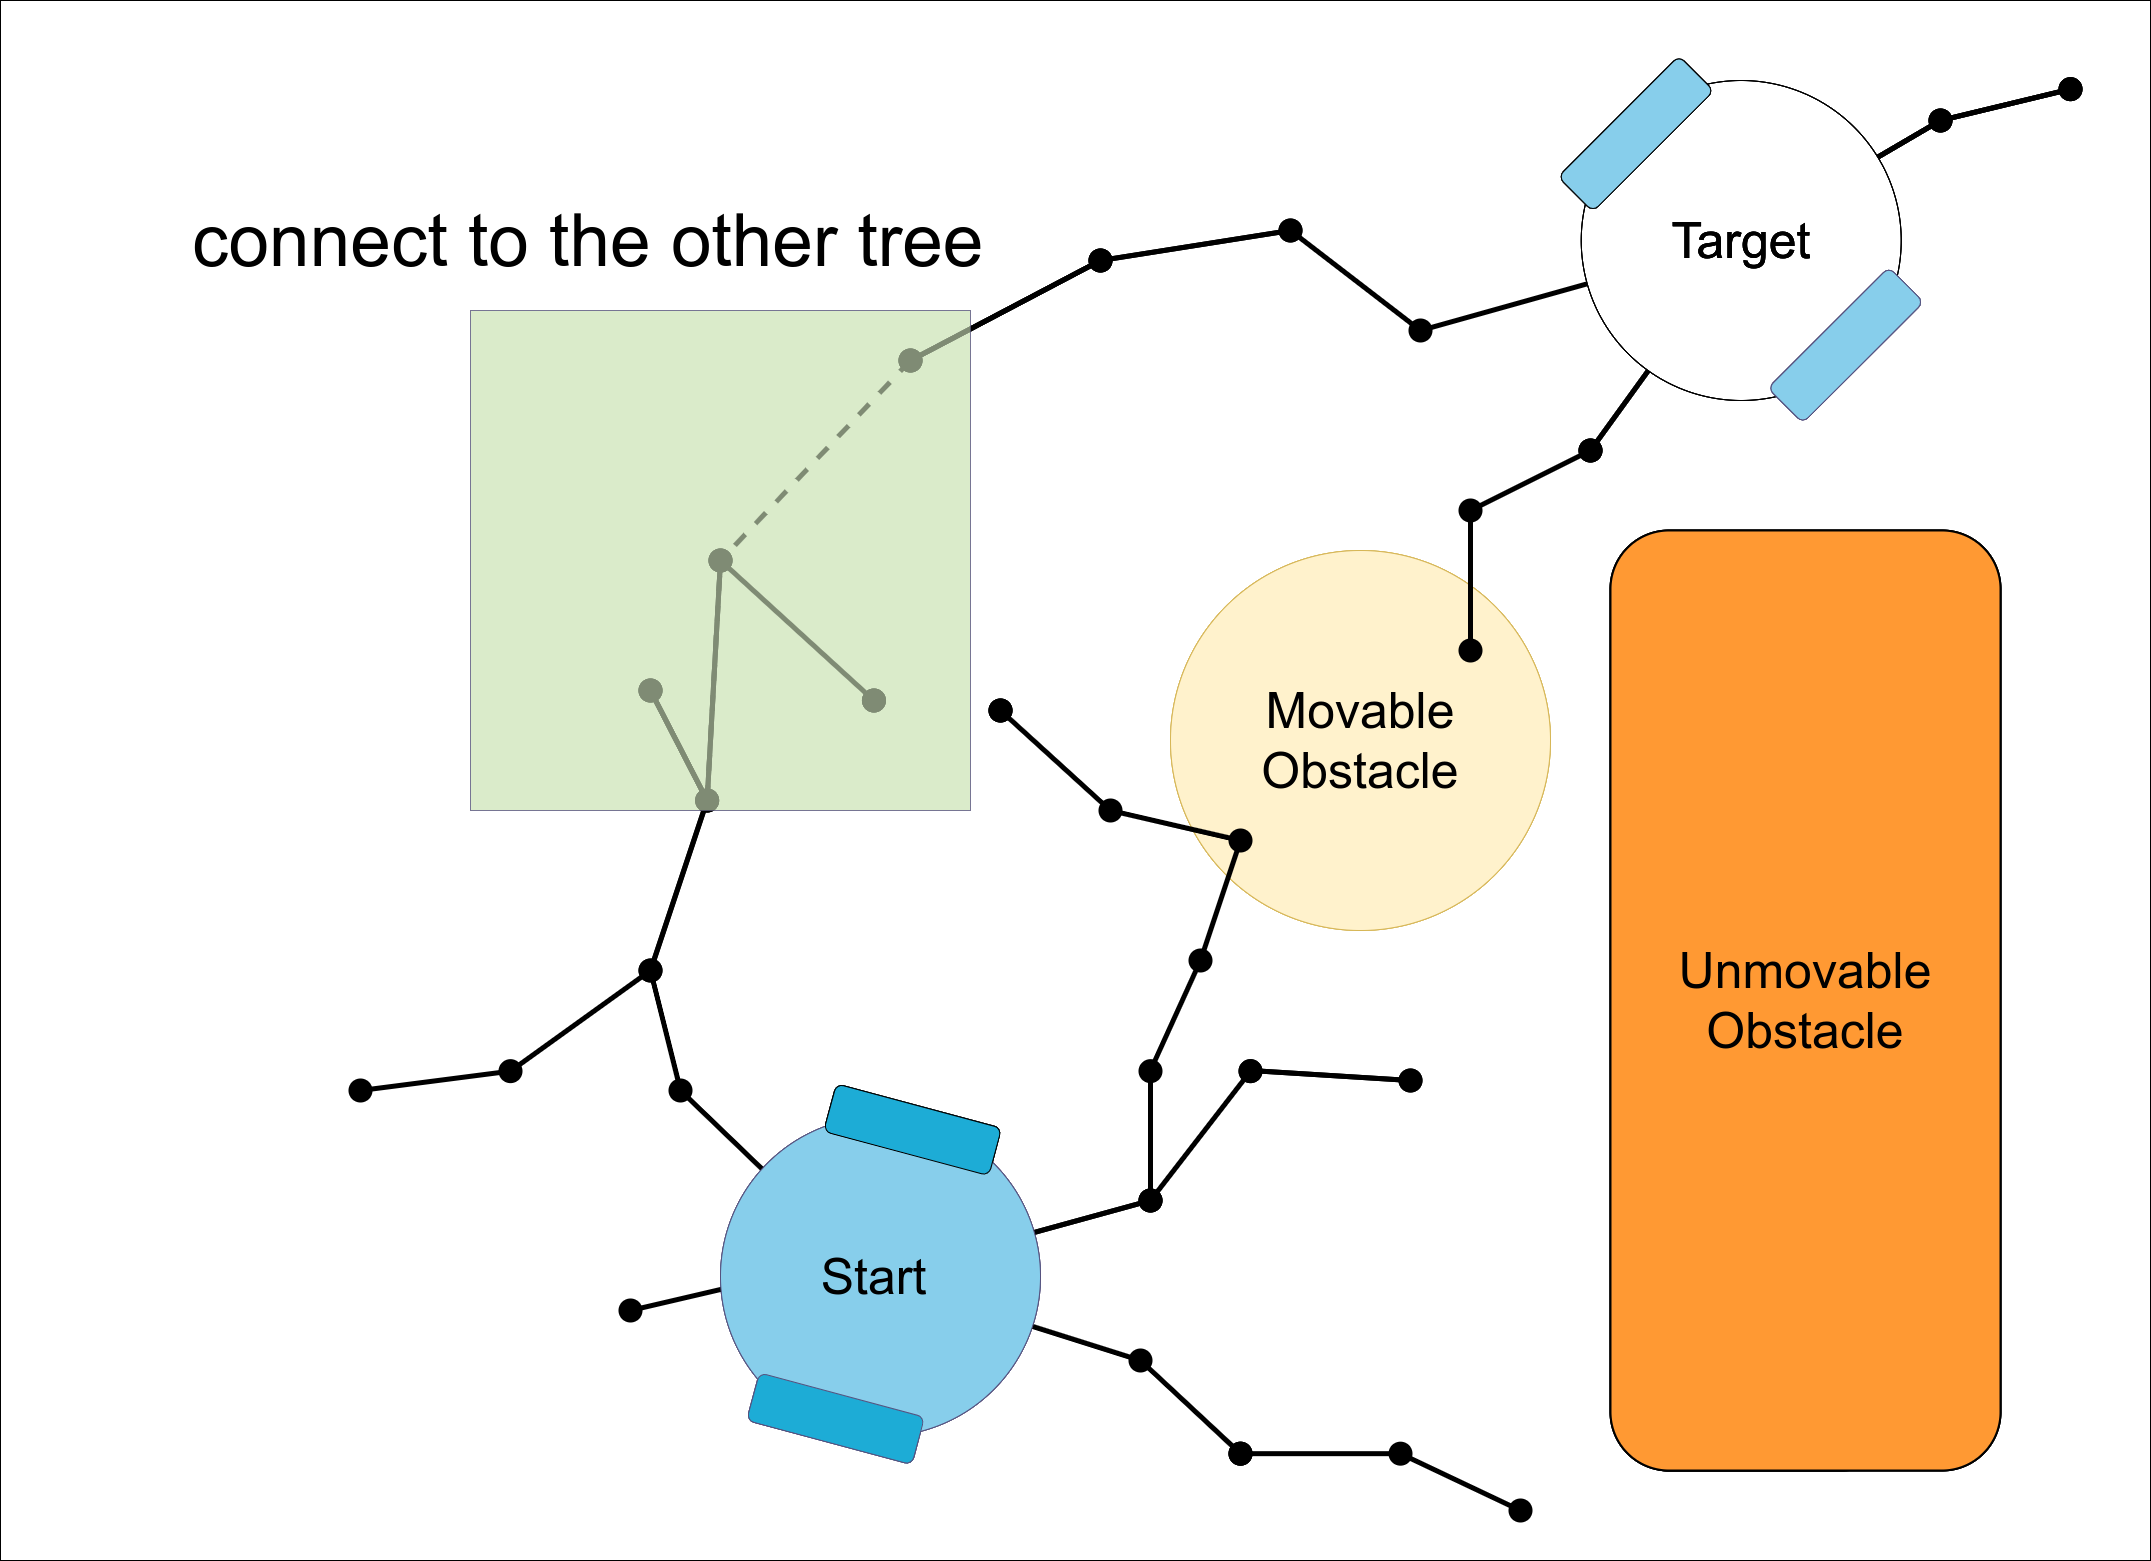
\includegraphics[width=0.93\textwidth, cfbox=my_green 5pt 0pt]{figures/mp/6mp_search_other_tree.drawio.png}
    \caption{A path from start to target configuration is found. \bs}
    \end{subfigure}

    \caption{Visualisation of the Double tree \acs{RRT*} motion planner that adds a single sample to the connectivity graph. The colour of the box surrounding subfigures corresponds to the coloured sections in \cref{pseudocode:proposed_rrt_star}. 3-dimensional configuration space displayed as 2-dimensional configuration space ($x$ and $y$ are visible, $\theta$ is not visible).}
    \label{fig:motion_planner_adding_one_sample}
\end{figure}


\begin{figure}[H]
    \centering
    \begin{subfigure}{.5\textwidth}
    \centering
    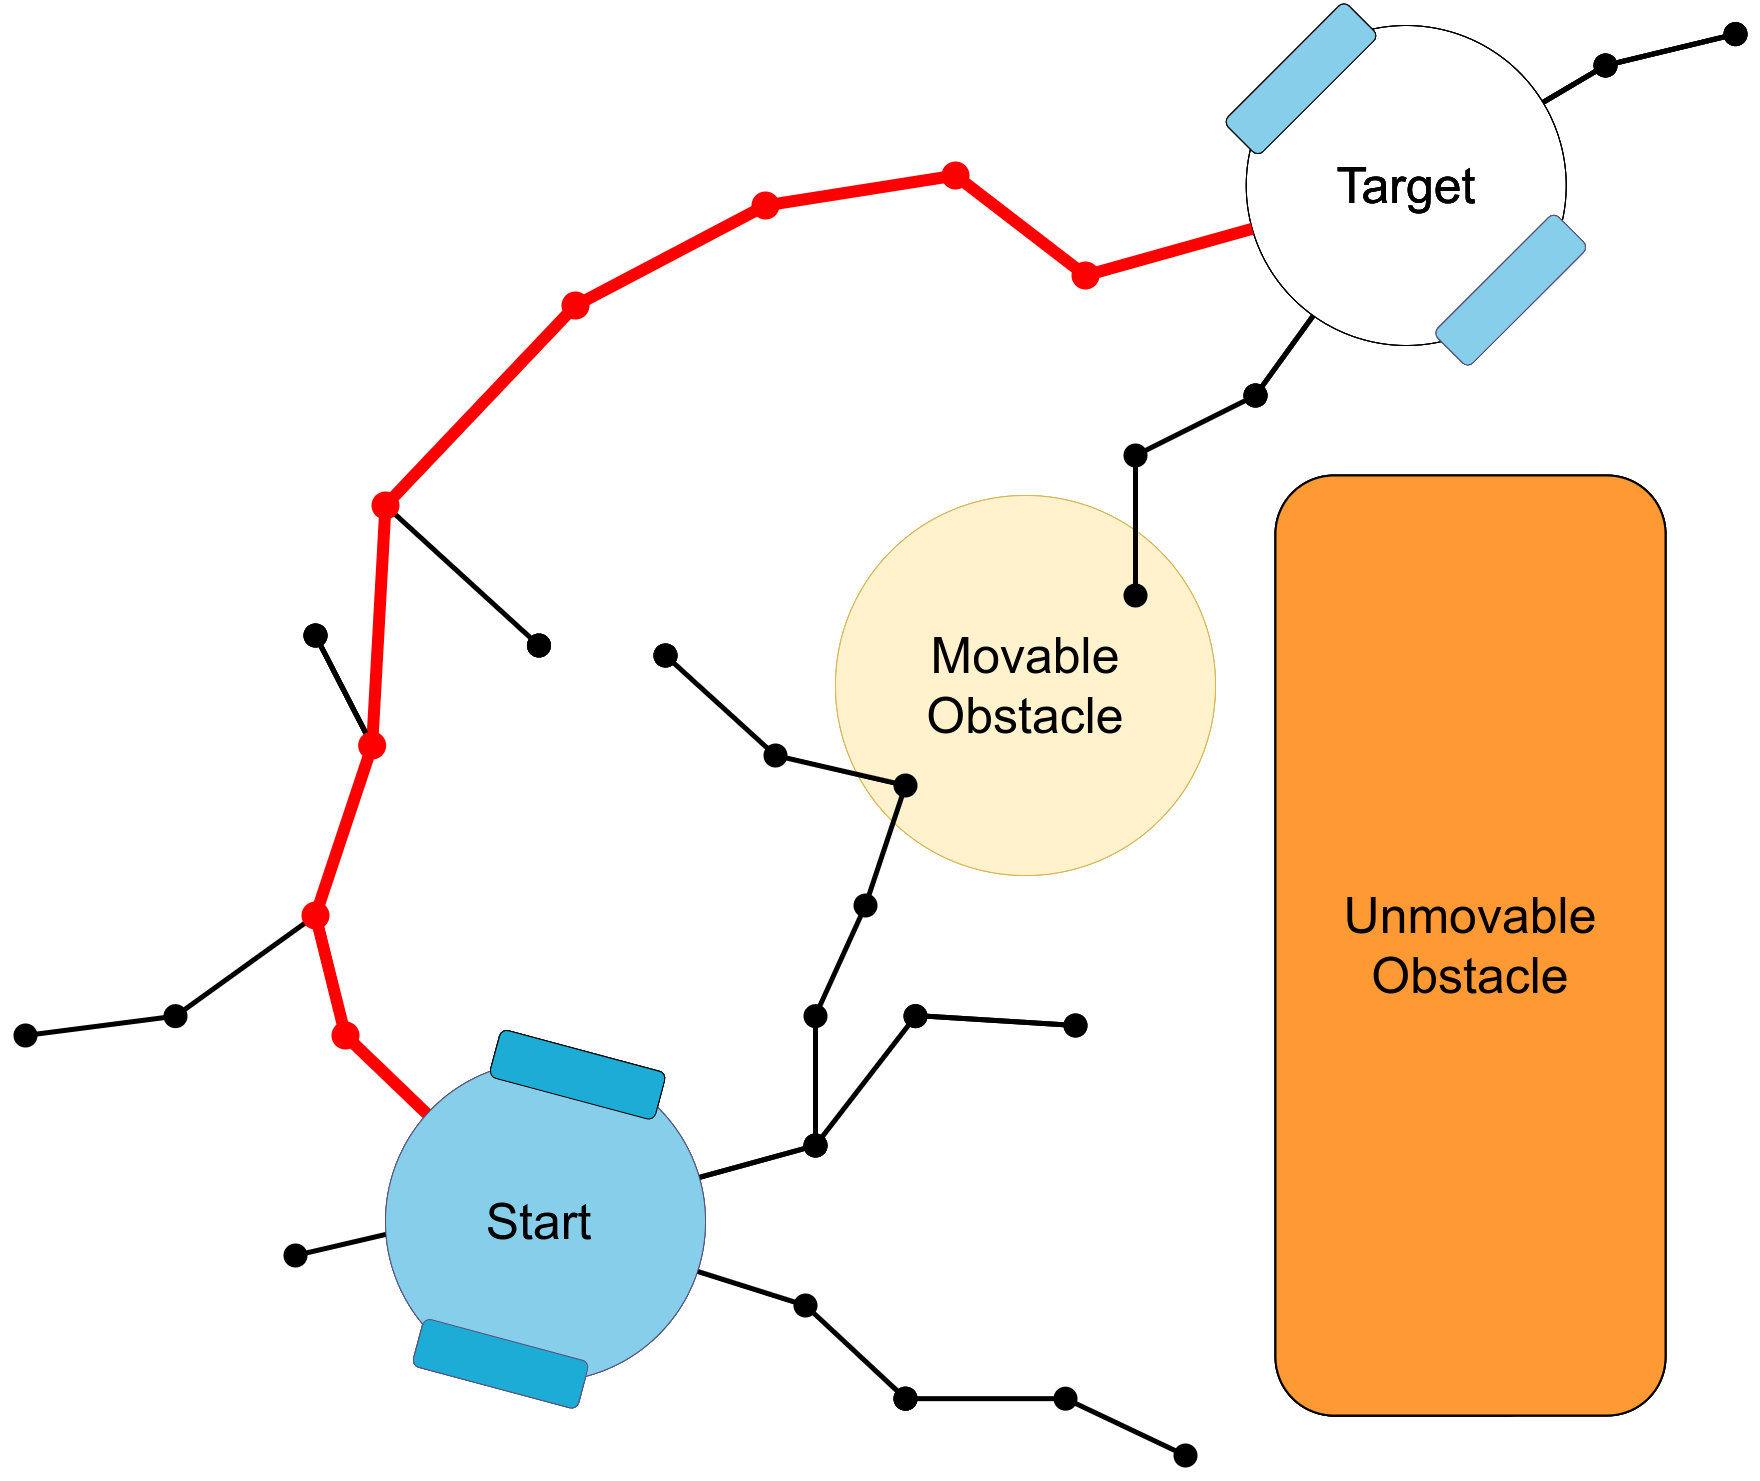
\includegraphics[width=0.75\textwidth]{figures/mp/7mp_path_found.drawio.png}
    \caption{The resulting configuration space after sample in \cref{fig:motion_planner_adding_one_sample}\\ was added. The path found is marked in red}
    \end{subfigure}%
    \begin{subfigure}{.5\textwidth}
    \hspace{-0.7cm}
    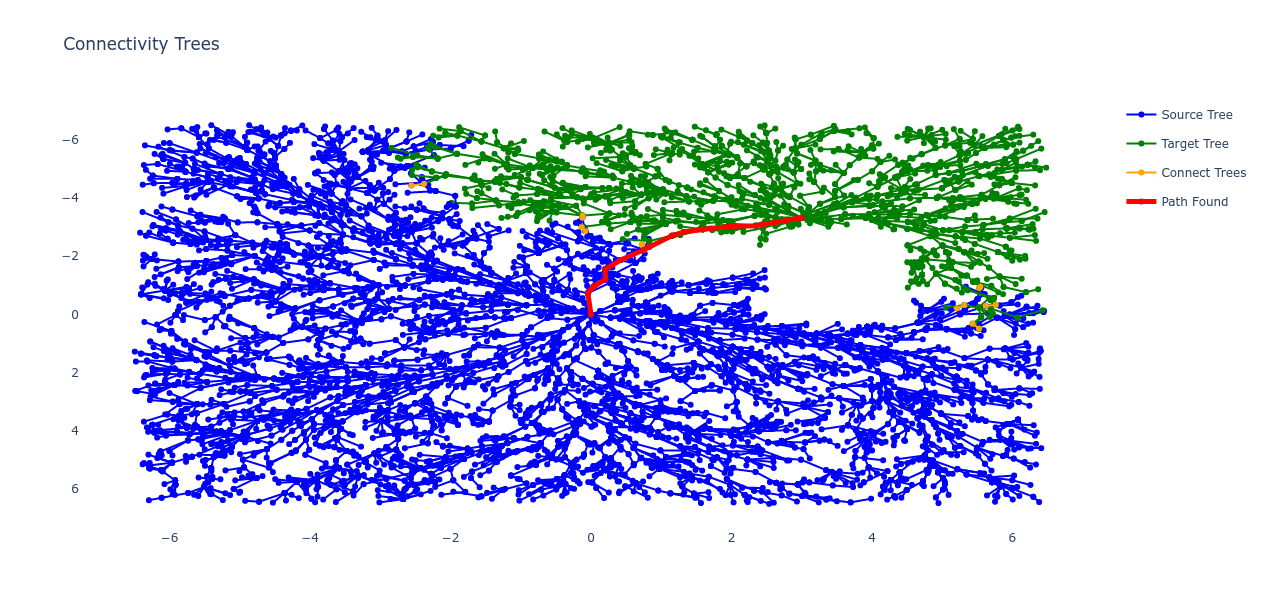
\includegraphics[width=1.1\textwidth]{figures/mp/mp_the_real_deal.png}
    \caption{A visualisation of the implemented \acs{RRT*} algorithm\\after a search from start to target}
    \end{subfigure}
    \label{fig:motion_planner_comparison}%
    \caption{Comparing schematic example to a visualisation of the real algorithm.}
\end{figure}

The result of adding an extra penalty for crossing unknown or movable subspace is that such subspaces are avoided if possible. If it is not possible to find a valid path, then movable or unknown subspaces are crossed, displayed in~\cref{fig:double_rrt_alg}. A path cannot be tracked by a controller if it crosses movable or unknown spaces, first, the object must be moved, and then the original path can be tracked. In~\cref{fig:double_rrt_alg} it can be seen that the motion planner cannot find a path around the movable object and is forced to add the cost to move the object. The added fixed cost for a path crossing through a movable or unknown object motivates the motion planner to find the shortest path around objects but prefers moving an object over making a large detour.\bs

\begin{figure}[H]
    \centering
    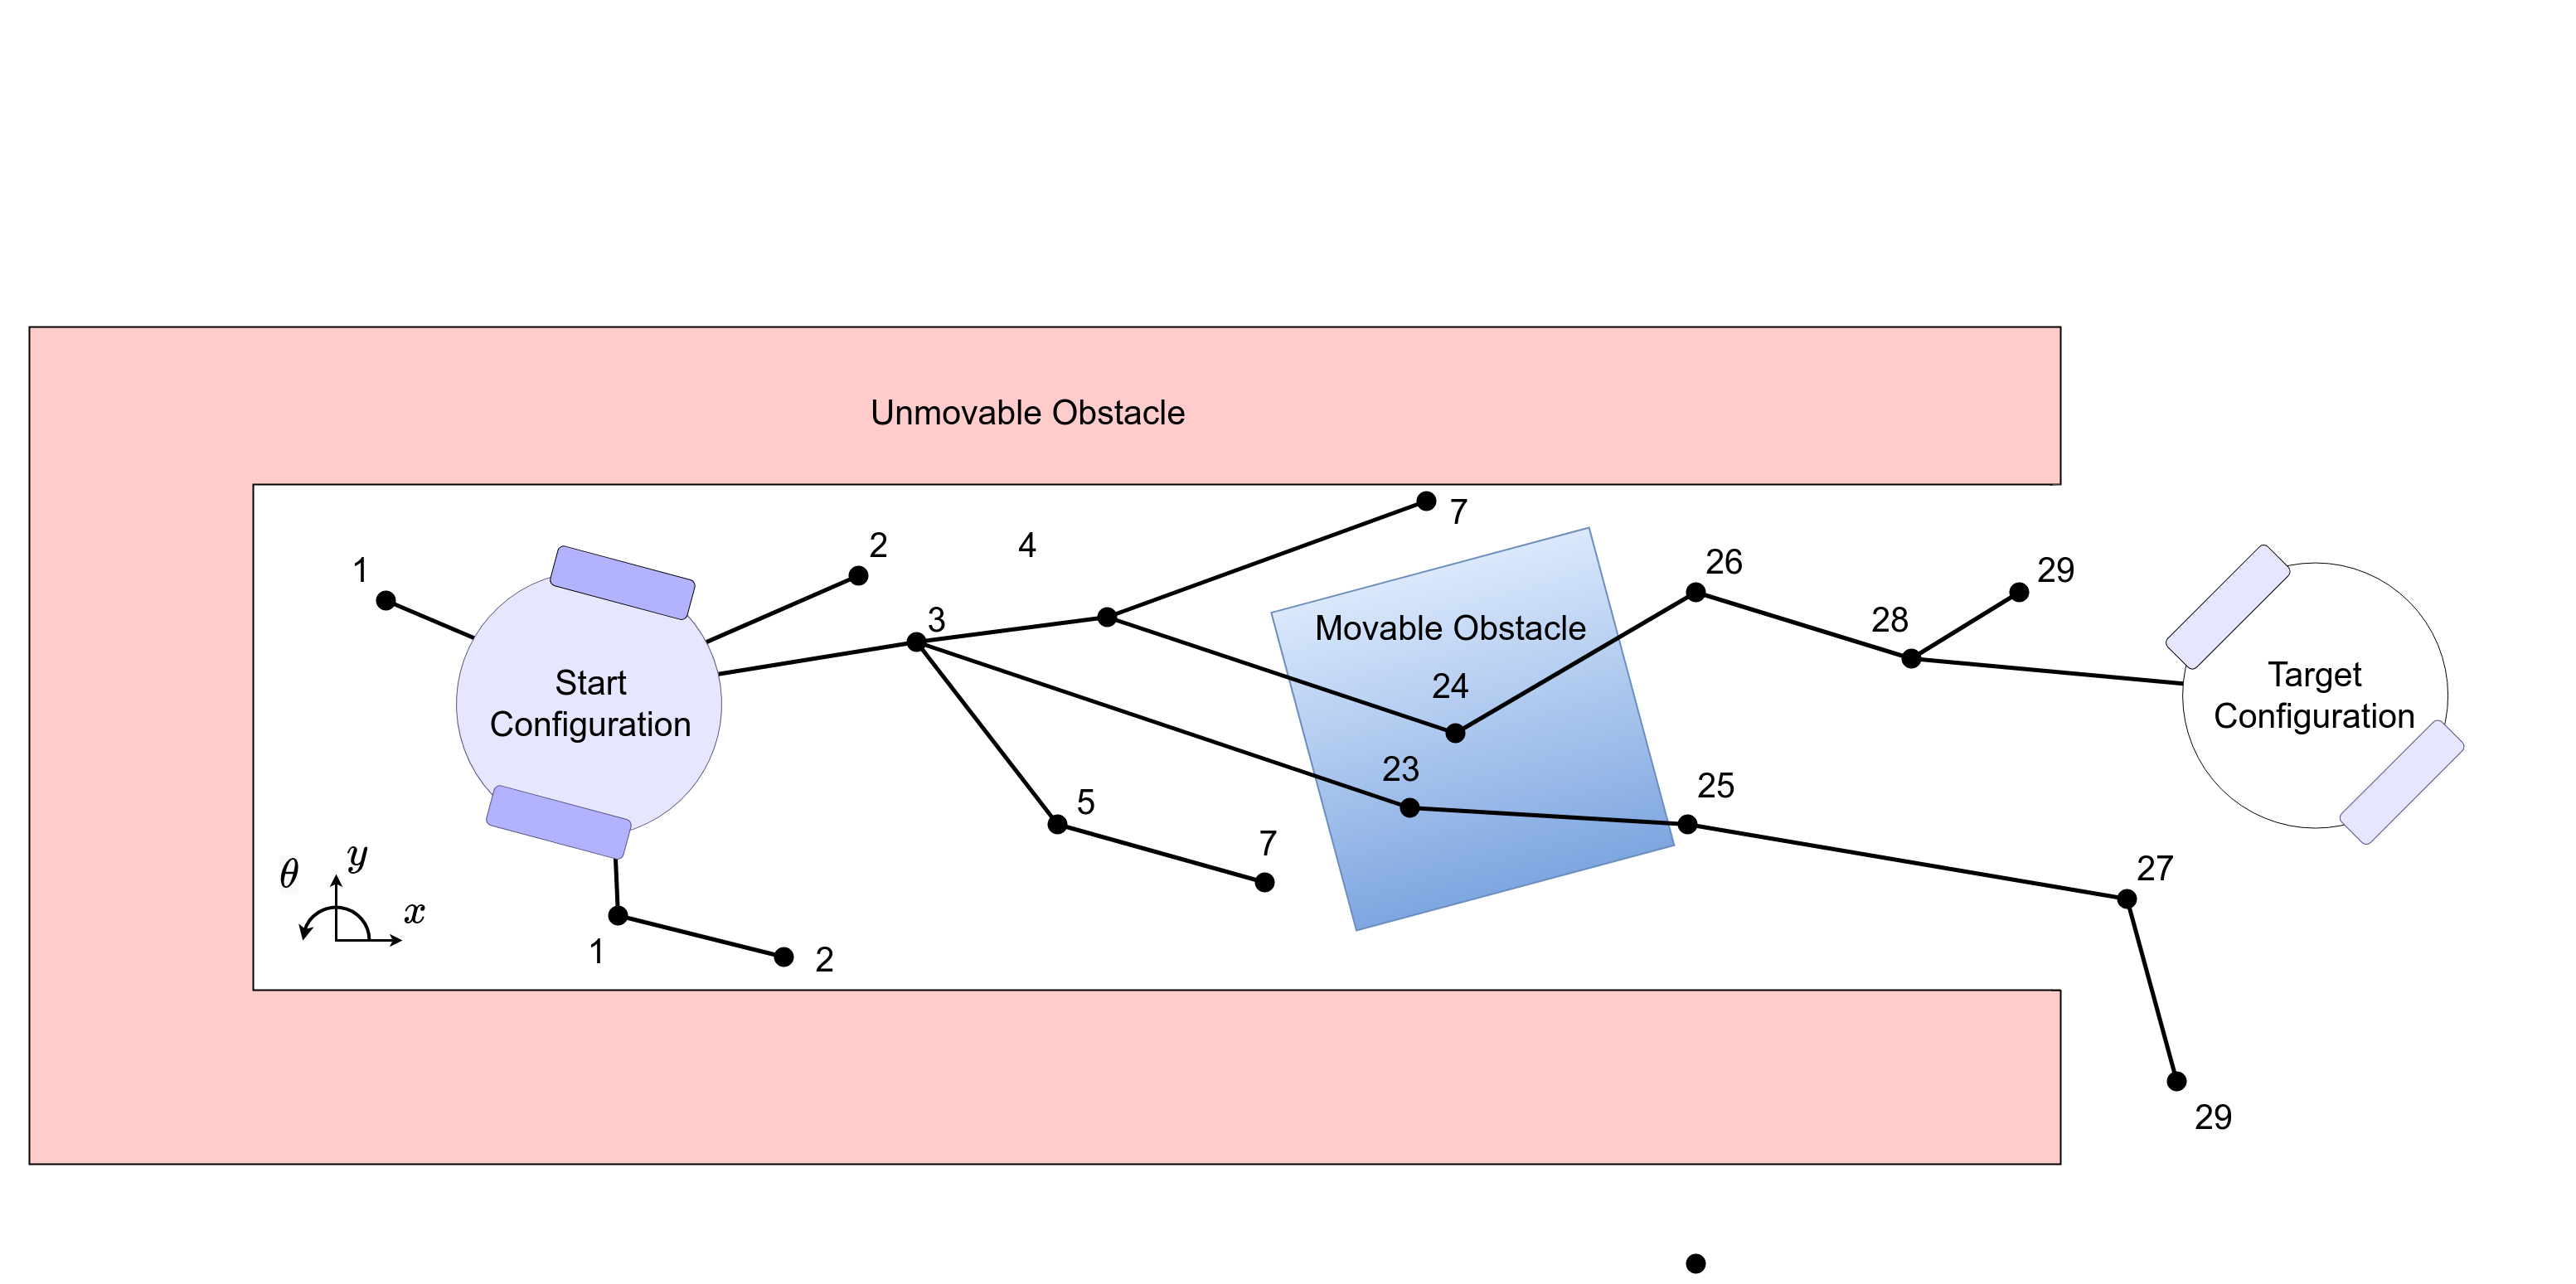
\includegraphics[width=0.9\textwidth]{figures/rrt_with_costs.png}
    \caption{Schematic view of the proposed double $\text{RRT}^*$ tree taking movable and\\unknown objects into account with cost to reach a sampled configuration displayed.}
    \label{fig:double_rrt_alg}
\end{figure}

The proposed motion planning algorithm searches the configuration space from the start connectivity tree and the target connectivity tree. Exploring faster compared to the single tree \ac{RRT*} algorithm. The proposed algorithm rewires nodes, resulting in lowering cost for existing paths. The proposed algorithm finds the optimal lowest-cost path with infinite sampling because of its ability to rewire nodes. The $LocalPlannerCheck$ provides feasible paths, such that the proposed algorithm yields paths that respect the system constraints. After all later on the system will be controlled to track the path. Now motion planning is discussed, manipulation will be discussed.

\subsection{Manipulation Planning}%
\label{subsec:manipulation_planning}
% Extending upon motion planning manipulation planning keeps track of 2 objects.
\todo[inline]{explain the manipulation planning extensions with a figure, no one is going to understand you otherwise.}
\todo[inline]{create manipulation planning subsection after implementation, code first, then write. Because writing is harder than coding}


\begin{figure}[H]
    \centering
    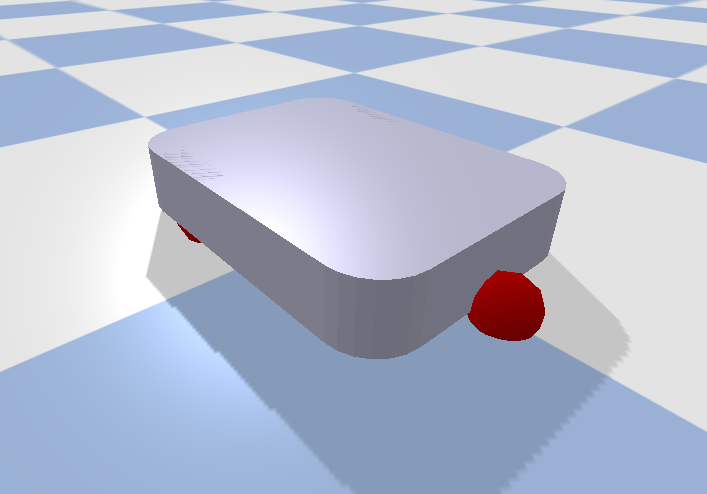
\includegraphics[width=5cm]{figures/boxer_robot}
    \caption{Speed comparison of increasingly difficult tasks}
    \label{fig:speed_comparison_planning}
\end{figure}
